\documentclass[a4paper,12pt,twoside]{article}
\usepackage[spanish]{babel}
\usepackage[utf8x]{inputenc}
\usepackage{graphicx} %para insertar graficos/imagenes
\usepackage{amsmath} %para escribir matrices
\usepackage{amsfonts} %para poner \mathbb
\usepackage{float} %me deja usar la H de 'here' en los graficos para ponerlos donde yo quiera
\usepackage{anysize} %me permite definir los margenes como quiera
\usepackage{multirow} %para tablas con multicolumna
\usepackage{fancyhdr} % activamos el paquete
\usepackage{dcolumn}
\usepackage{multirow}
\usepackage{booktabs}


\usepackage{lscape}



\usepackage{varioref}



\usepackage{fixme}
\fxsetup{
    status=draft,
    author= ,
    layout=inline, % also try footnote or pdfnote
}

\newcommand{\grad}{$^\circ$}

\newcommand{\codigoMateria}{66.10}
\newcommand{\nombreMateria}{Circuitos Electrónicos II}
\newcommand{\nroTP}{1}
\newcommand{\descripcionTP}{Informe de Avance del Proyecto}
\newcommand{\tituloTP}{Amplificador Clase G}
\newcommand{\facultad}{Facultad de Ingeniería}
\newcommand{\universidad}{Universidad de Buenos Aires}
\newcommand{\docentes}{José Alberto Bertuccio\\Federico D'Angiolo}

\pagestyle{fancy} % seleccionamos un estilo
\fancyhead{}
\fancyfoot{}
\lhead{\nombreMateria \, (\codigoMateria)} % texto izquierda de la cabecera
\rhead{\facultad} % texto centro de la cabecera
\cfoot{\thepage}

\marginsize{2cm}{2cm}{1cm}{1.5cm} %izquierda, derecha, arriba, abajo

\newcommand{\Direcrotio}{./}
\newcommand{\HRule}{\rule{\linewidth}{1mm}}


% Símbolos de las unidades
% Se utiliza el comando \ensuremath{~} por seguridad
% Incluyo también gensymb que añade los comandos:
%\degree, \celsius, \perthousand, \micro and \ohm
%	º		ºC			o/oo		µ			Ω

\usepackage{gensymb}

% VOLT
\newcommand{\nV}{\ensuremath{~\mathrm{nV}}}
\newcommand{\uV}{\ensuremath{~\mu\mathrm{V}}}
\newcommand{\mV}{\ensuremath{~\mathrm{mV}}}
\newcommand{\volt}{\ensuremath{~\mathrm{V}}}

% HERTZ
\newcommand{\hz}{\ensuremath{~\mathrm{Hz}}}
\newcommand{\hertz}{\ensuremath{~\mathrm{Hz}}}
\newcommand{\Hz}{\ensuremath{~\mathrm{Hz}}}
\newcommand{\khz}{\ensuremath{~\mathrm{kHz}}}
\newcommand{\kHz}{\ensuremath{~\mathrm{kHz}}}
\newcommand{\Mhz}{\ensuremath{~\mathrm{MHz}}}
\newcommand{\MHz}{\ensuremath{~\mathrm{MHz}}}

% FARAD
\newcommand{\pF}{\ensuremath{~\mathrm{pF}}}
\newcommand{\nF}{\ensuremath{~\mathrm{nF}}}
\newcommand{\uF}{\ensuremath{~\mu\mathrm{F}}}
\newcommand{\mF}{\ensuremath{~\mathrm{mF}}}
\newcommand{\farad}{\ensuremath{~\mathrm{F}}}

% OHM
%\newcommand{\ohm}{\ensuremath{~\Omega}}
\newcommand{\nohm}{\ensuremath{~\mathrm{n}\ohm}}
\newcommand{\uohm}{\ensuremath{~\mu\ohm}}
\newcommand{\mohm}{\ensuremath{~\mathrm{m}\ohm}}
\newcommand{\kohm}{\ensuremath{~\mathrm{k}\ohm}}
\newcommand{\Mohm}{\ensuremath{~\mathrm{M}\ohm}}

% HENRY
\newcommand{\uHy}{\ensuremath{~\mu\mathrm{Hy}}}
\newcommand{\nHy}{\ensuremath{~\mathrm{nHy}}}
\newcommand{\mHy}{\ensuremath{~\mathrm{mHy}}}
\newcommand{\henry}{\ensuremath{~\mathrm{Hy}}}

% AMPERE
\newcommand{\fA}{\ensuremath{~\mathrm{fA}}}
\newcommand{\uA}{\ensuremath{~\mu\mathrm{A}}}
\newcommand{\nA}{\ensuremath{~\mathrm{nA}}}
\newcommand{\mA}{\ensuremath{~\mathrm{mA}}}
\newcommand{\amper}{\ensuremath{~\mathrm{A}}}

% SEGUNDOS
\newcommand{\nS}{\ensuremath{~\mathrm{ns}}}
\newcommand{\uS}{\ensuremath{~\mu\mathrm{s}}}
\newcommand{\mS}{\ensuremath{~\mathrm{ms}}}
\newcommand{\seg}{\ensuremath{~\mathrm{s}}}

% WATTS
\newcommand{\mW}{\ensuremath{~\mathrm{mW}}}
\newcommand{\watt}{\ensuremath{~\mathrm{W}}}

% DECIBELES
\newcommand{\dB}{\ensuremath{~\mathrm{dB}}}
\newcommand{\dBm}{\ensuremath{~\mathrm{dBm}}}

% señal
\newcommand{\vs}[1]{%
\ensuremath{~v_{\mathrm{#1}}}%
}
\newcommand{\is}[1]{%
\ensuremath{~i_{\mathrm{#1}}}%
}

\usepackage[font=footnotesize, labelfont=bf,margin=2.2cm]{caption}


% ctes
\newcommand{\VA}{\ensuremath{~\mathrm{V}_{\mathrm{A}}}}
\newcommand{\VT}{\ensuremath{~\mathrm{V}_{\mathrm{T}}}}
\newcommand{\Vth}{\ensuremath{~\mathrm{V}_{\mathrm{th}}}}
\newcommand{\VCC}{\ensuremath{~\mathrm{V}_{\mathrm{CC}}}}
\newcommand{\VBB}{\ensuremath{~\mathrm{V}_{\mathrm{BB}}}}
\newcommand{\VDD}{\ensuremath{~\mathrm{V}_{\mathrm{DD}}}}
\newcommand{\VGG}{\ensuremath{~\mathrm{V}_{\mathrm{GG}}}}
\newcommand{\VSS}{\ensuremath{~\mathrm{V}_{\mathrm{SS}}}}
\newcommand{\RB}{\ensuremath{~\mathrm{R}_{\mathrm{B}}}}
\newcommand{\RC}{\ensuremath{~\mathrm{R}_{\mathrm{C}}}}
\newcommand{\RE}{\ensuremath{~\mathrm{R}_{\mathrm{E}}}}
\newcommand{\RL}{\ensuremath{~\mathrm{R}_{\mathrm{L}}}}
\newcommand{\RG}{\ensuremath{~\mathrm{R}_{\mathrm{G}}}}
\newcommand{\RD}{\ensuremath{~\mathrm{R}_{\mathrm{D}}}}
\newcommand{\RS}{\ensuremath{~\mathrm{R}_{\mathrm{S}}}}
\newcommand{\Rs}{\ensuremath{~\mathrm{R}_{\mathrm{s}}}}
\newcommand{\R}[1]{%
\ensuremath{~\mathrm{R}_{\mathrm{#1}}}%
}
\newcommand{\I}[1]{%
\ensuremath{~\mathrm{I}_{\mathrm{#1}}}%
}
\newcommand{\V}[1]{%
\ensuremath{~\mathrm{V}_{\mathrm{#1}}}%
}
\newcommand{\Ip}[1]{%
\ensuremath{~\hat{\mathrm{I}}_{\mathrm{#1}}}%
}
\newcommand{\Vp}[1]{%
\ensuremath{~\hat{\mathrm{V}}_{\mathrm{#1}}}%
}
\newcommand{\ip}[1]{%
\ensuremath{~\hat{i}_{\mathrm{#1}}}%
}
\newcommand{\vp}[1]{%
\ensuremath{~\hat{v}_{\mathrm{#1}}}%
}
\newcommand{\A}[1]{%
\ensuremath{~\mathrm{A}_{\mathrm{#1}}}%
}
\newcommand{\nada}{\quad{}}


\newenvironment{items}{
\begin{itemize}
  \renewcommand{\labelitemi}{$\bullet$}
  \setlength{\itemsep}{3pt}
  \setlength{\parskip}{1pt}
  \setlength{\parsep}{1pt}
}{
\end{itemize}}



\begin{document}



\begin{titlepage}

\thispagestyle{empty}

\begin{center}


\includegraphics[scale=0.15]{fiuba}\\[0.1cm]
\textsc{\universidad}\\[0.2cm]
\large{\textsc{\facultad}}\\[0.2cm]

\end{center}

\vfill

\begin{center}
\underline{\Large{\nombreMateria\, (\codigoMateria)}}
\end{center}

\vfill
\begin{center}

\end{center}
\vfill

\begin{center}
\Huge{\textsc{ \tituloTP }}\\[.5cm]
	\begin{figure}[H]
		\centering
		%\includegraphics[width=.5\textwidth]{bessel}
	\end{figure}\HRule \\[0.1cm]
\Huge{\textbf{\descripcionTP}}\\[0.01cm]
\HRule\\[0.3cm]
\end{center}

\vfill



\begin{tabbing}
	FECHA: \today\\
\\
	INTEGRANTES:\hspace{-1cm}\=\+\hspace{1cm}\=\hspace{6cm}\=\\
		Gomez, Cristian	\>\>- \#89968\\
			\>\footnotesize{$<$crisgvenezia@gmail.com$>$}\\
		Pollitzer, Ivan Gustavo	\>\>- \#22922\\
			\>\footnotesize{$<$igpollitzer@gmail.com$>$}\\
		Carballeda, Ignacio	\>\>- \#91646\\
			\>\footnotesize{$<$carballeda.ignacio@gmail.com$>$}\\

\end{tabbing}

\begin{flushleft} \large
\emph{Docentes:}\\[.2cm]
\end{flushleft}
\begin{tabbing}
\docentes\\[.5cm]
\end{tabbing}

\vfill

\hrule
\vspace{0.2cm}

\noindent\small{\codigoMateria\, --- \nombreMateria \hfill \facultad}

\end{titlepage}


\newpage
\vfill
\tableofcontents
\vfill

%\listoffixmes

\newpage

\section{Actividades desarrolladas}

\subsection{Diseño conceptual}

\subsubsection{Objetivo y requerimientos de usuario}

El objetivo es amplificar una señal de audio que será reproducida en un parlante.  Debe proveer al usuario con una buena calidad de sonido con volumen alto sin consumir mucha más energía de la necesaria ni ser muy grande y pesado. Es decir, debe tener baja distorsión, alta relación señal-ruido (SNR), eficiencia razonable y buena ganancia y potencia máxima de salida.



\subsubsection{Especificaciones}

\bigskip

\begin{itemize}
	\item Máxima Potencia de Salida:  $100\watt$ RMS @ $8\ohm$
	\item Salida clase G
	\item THD: $< 0.01 \% @ 1kHz$, $<0.02 \% @ 10kHz,$ a $100W RMS/8\Omega$ y $1W RMS/8\Omega$
	\item Slew Rate: $>15\frac{V}{\mu S}$
	\item Impedancia de entrada: $10\kohm$
	\item Sensibilidad: $1\volt$ RMS @ $8\Omega$
	\item Ancho de banda: $10 Hz-30kHz$
	\item Factor de amortiguamiento: $>200$
	\item Ancho de banda de potencia: $>30kHz$
	\item Alimentación: 
	\begin{itemize}
		\item Baja tensión: $ +/-15\volt$ al $5\%$
		\item Alta tensión: $ +/-50\volt$ al $5\%$
	\end{itemize}
\end{itemize}

\paragraph{Máxima excursión} Para una salida senoidal de $100W RMS$, su potencia pico es $200W = \frac{V_{max}^2}{R_L}$ que, con carga $R_L=8\Omega$ da una tensión pico de $V_{max}=40V$. A esta tensión se llega cuando la entrada es la sensibilidad especificada, $1V RMS @8\Omega$, que se corresponde a $1V pico$. Estos $40V$ serán la máxima excursión, la tensión máxima en la que el amplificador garantiza que no haya recortes considerables.

\paragraph{Nota sobre el slew-rate} El mayor ritmo de crecimiento para señales que cumplen con las especificaciones de ancho de banda $30kHz$ y máxima excursión $40V$ se da cuando la senoide cruza por cero, y su pendiente es $2 \pi \times 30kHz\times 40V\cong 7.5\frac{V}{\mu s}$. El slew rate especificado ($15\frac{V}{\mu s}$) duplica este valor mínimo.


\subsubsection{Diseño general}

Un amplificador típico consta, basicamente, de 3 etapas: una de entrada, diferencial,  una intermedia, de ganancia de tensión, y una de salida, de ganancia de corriente. Esta última etapa es la responsable de proveer la potencia y la que determina la eficiencia, tamaño y peso del amplificador.


\paragraph{Etapa de entrada}
La etapa de entrada puede ser de distintas maneras, puede ser una etapa de amplificación simple, o diferencial. Nosotros escogimos la topografía diferencial, debido a que nos provee una Relacion de Rechazo de Modo Común elevada. Es decir, atenúa las señales que sean iguales  por ambas entradas, y aumenta las que sean opuestas. Las señales iguales, pueden darse por distintos tipos de ruido, que es lo que queremos evitar, mientras que las opuestas, son la señal que quermos amplificar. Inicialmente consideramos una típica topología diferencial, de colectores acoplados. Pero como los transistores no son componentes lineales, propusimos agregar otro par diferencial, en paralelo, con componentes complementarios; es decir, donde originalmente usamos transistores NPN, colocamos PNP, y viceversa. De esta forma, la simetría cancela alinealidades y se reduce la distorsión. Esto llevó a luego intentar mantener una simetría total en todo el circuito. Otra opción de diseño más, es la de la carga de los pares diferenciales. Estos pueden ser activas o pasivas. Por lo general, se elige una carga de tipo activa, como por ejemplo, una fuente de corriente espejo, porque da una menor distorsión, pero en nuestro caso, elegimos un amplificador tipo cascode, con una carga pasiva, porque necesitamos la carga para polarizar la etapa siguiente, donde explicaremos el motivo.

\paragraph{Etapa de amplificación de tensión (VAS).}

Por lo general, la etapa de amplificación suele estar compuesta por un simple amplificador de configuración Emisor Común, entrando a la etapa de salida, por debajo del multiplicador de $V_{be}$, y polarizado por una fuente de corriente de colector. Esta etapa puede modificarse, agregando una etapa colector común, antes del amplificador (EF VAS), para separar la etapa de entrada; esto mejora la distorsión. También se puede modificar para que la salida del VAS no sea por debajo del multiplicador de Vbe, sino por el medio, para disminuir el offset a la salida, previo a la realimentación, y disminuir la distorsión. El inconveniente de este modo es que se necesitan dos fuentes de corriente más, ya que el modo anterior, aprovecha la fuente de polarización del EF VAS, para polarizar, también, el multiplicador de Vbe. En nuestro caso, con el cambio a 2 pares diferenciales, duplicamos la etapa EF VAS, complementariamente, y se conectan a la etapa de salida, por arriba y por abajo del multiplicador de $V_{be}$. Como en este caso, cada uno de los dos EF VAS hace de carga del otro, los EF VAS no tienen fuente de polarización, entonces se necesita que la etapa diferencial tenga una carga resistiva, para fijar la tensión de base de los EF VAS. Si hubieramos usado una carga tipo fuente espejo, habríamos logrado que la corriente en las ramas del par diferencial fuera igual, pero sin fijar ninguna tensión para polarizar la base de los EF VAS.

\paragraph{Etapa de salida}
Esta etapa es la responsable de amplificar la potencia de la señal. Es decir, debe tener \textbf{alta eficiencia}, y \textbf{bajos niveles de distorsión}. Además, se busca \textbf{minimizar la impedancia de salida} para mantener un \textbf{alto factor de amortiguamiento} y evitar que el rebote acústico afecte el comportamiento del amplificador. 
La etapa de salida clase G está compuesto por dos o más niveles de alimentación que permiten incrementar la eficiencia del amplificador con respecto al clase B. Esto se logra ya que con tensiones bajas, se utilizará una fuente de tensión menor, preservando la máxima excursión posible sobre la carga que ofrece un clase B alimentado con la fuente de tensión mayor. Para señales con picos de baja amplitud en relación al valor medio, la mejora en la eficiencia es modesta. Sin embargo, en el caso en que la señal tenga picos considerables con respecto a su valor medio, la mejora es notable. Un punto importante, a la hora de diseñar una etapa de salida clase G, es la tensión de los rieles internos. Tomamos del libro de Douglas Self, los estudios realizados considerando los casos en los cuales la tensión de riel interno es de 30 y 60\% del externo, y se observó que los beneficios en cuanto a eficiencia, del segundo caso, son pocos. En cambio, en el caso de rieles internos de 30\% respecto de los externos, la eficiencia aumenta considerablemente. Otro detalle de diseño, es la del multiplicador de Vbe doble. El multiplicador de Vbe más simple, tiene un transistor, y 2 resistencias, con las que forma el salto de potencial necesario para eliminar el problema de cruce por 0 de la etapa de salida. En este caso, se usan 2 transistores complementarios, con la misma idea que el del doble par diferencial, para que el corrimiento de tensión del multiplicador de Vbe sea lo más lineal posible.

\paragraph{Realimentador global}


Debido a la complejidad del circuito, cumplir con todas las especificaciones a lazo abierto es altamente complejo y requiere demasiada precisión en el cálculo y elección de componentes. Esto derivaría en un circuito altamente complejo y costoso. Es por este motivo que se emplea el realimentador.

Dado que en un amplificador de audio se busca que la salida sea una versión de escalada de la señal de entrada, se busca tomar una muestra de la misma, y compararla con la señal de entrada. 

Suponiendo que la ganancia a lazo abierto del circuito es mucho mayor que la ganancia del realimentador, este último es el encargado de fijar la ganancia a lazo cerrado, siendo la misma $A_v \simeq \frac{1}{f}$, y $f$ la ganancia del realimentador.

Una ventaja de esta técnica es que ayuda a que el amplificador se asemeje a un amplificador de tensión ideal, ya que aumenta la resistencia de entrada, mientras que disminuye la de salida. 

La realimantación es muy beneficiosa siempre que sea negativa. Dado que el sistema introduce defasajes, para ciertas frecuencias la realimentación pasa de ser negativa a ser positiva (esto haría que las diferencias entre la señal de salida real y deseada se amplifiquen en lugar de reducirse). Para evitar que el circuito se vuelva inestable, es necesario que para las frecuencias donde se invierte la fase, el circuito pase de amplificar a atenuar. Si esto no ocurre naturalmente, es necesario agregar componentes adicionales para compensar el circuito y evitar que se vuelva inestable

Otro factor a tener en cuenta, es que puede darse la aparición de frecuencias en la salida del circuito fuera del rango de las que se presentan naturalmente en la entrada (en este caso 20Hz - 20kHz por tratarse de audio). También para eliminar estos inconvenientes es que el sistema debe ser compensado.

El uso de realimentación global permite mejorar notablemente casi todas las especificaciones del amplificador y simplificar su diseño. En este caso, como el objetivo es armar un amplificador de tensión, utilizamos un circuito realimentador Serie-Paralelo. El factor de realimentación queda definida por las especificaciones de sensibilidad y potencia RMS para una carga de $8\Omega$. La ganancia del amplificador debe ser de $29dB$ y por lo tanto el realimentador debe atenuar $-29dB$.



\subsubsection{Diagrama en bloques}



\begin{figure}[H]
	\centering
	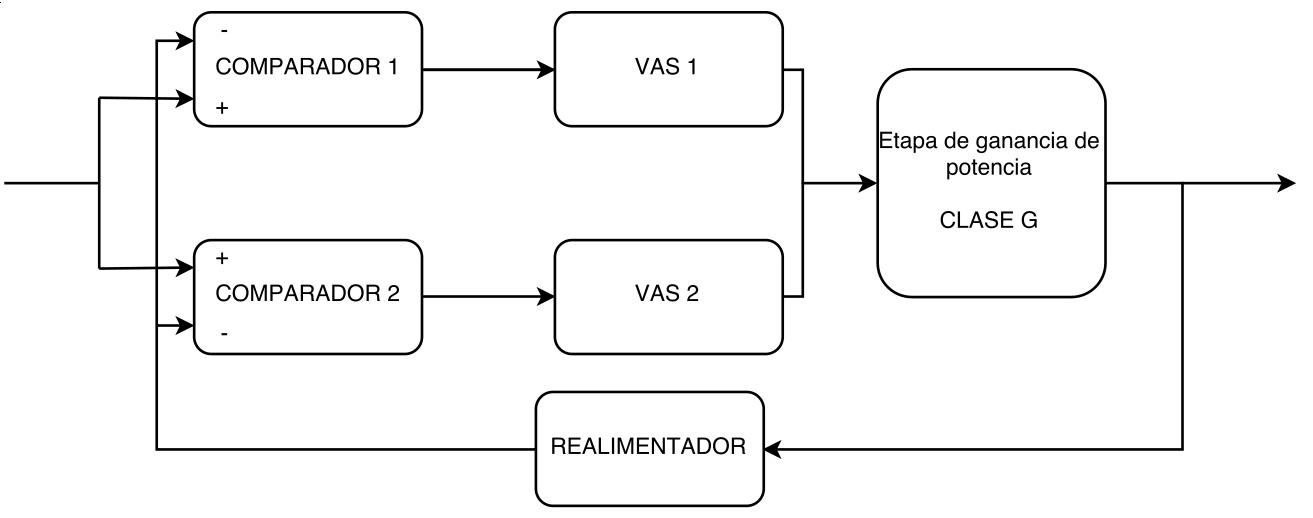
\includegraphics[width=0.9\textwidth]{img/bloques}
	\caption{Diagrama en bloques del amplificador clase G}
	\label{fig:ampli_bloques}
\end{figure}

Visto como un modelo de idealizado de Amplificador y realimentación, el circuito se presenta de la siguiente manera:

\begin{figure}[H]
	\centering
	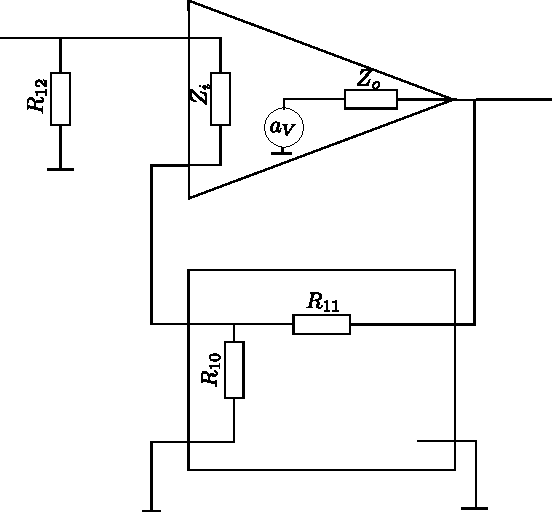
\includegraphics[width=0.5\textwidth]{img/realimentacion}
	\caption{Modelo amplificador-realimentación}
	\label{fig:ampli_realimentacion}
\end{figure}

Este dibujo muestra como el amplificador se encuentra realimentado con una topología serie-paralelo, midiendo tensión a la salida, y sumando tensión a la entrada, resultando un amplificador de ganancia de tensión estabilizado en tensión. Para hallar los valores de impedancia de entrada y salida, primero debemos reflejar las resistencias $R_{10}$ y $R_{11}$, como vemos en el siguiente dibujo.

\begin{figure}[H]
	\centering
	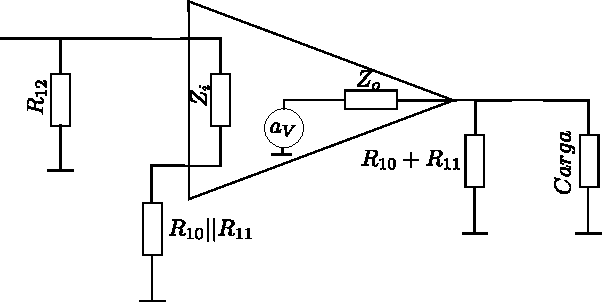
\includegraphics[width=0.5\textwidth]{img/reflejo}
	\caption{Modelo amplificador-reflejando resistencias}
	\label{fig:ampli_reflejo}
\end{figure}

El amplificador tiene una amplificación de tensión, de aproximadamente $80$ dB, con una elevada impedancia de entrada, y una impedancia de salida de aproximadamente $6\;\Omega$.
La realimentación tiene un valor de $\frac{1}{f} = \frac{R_{10}}{R_{10} + R_{11}} \rightarrow f = 0.035$, resultando $1+a_V\times f = 9\mathrm{K} \times 0.035 = 318.77$. En cuanto a la impedancia de entrada, $R_{11}$ y $R_{10}$ se reflejan en paralelo entre ellas, en serie a la impedancia de entrada del amplificador $Z_i$. Dada la relación entre las resistencias, $R_{11}$ resulta despreciable, y a su vez, $R_{10}$ resulta despreciable en serie con $Z_i$, que resulta despreciable, en paralelo con $R_{12}$, de $10\; \mathrm{K}\Omega$. Para la resistencia de salida, tenemos la resistencia reflejada $R_{10} + R_{11}$, que es despreciable en paralelo con $Z_o || R_{Carga} = 3.42\; \Omega$. Luego $\frac{3.42}{(1 + a_V \times f)} = 0.01\; \Omega$, que es la impedancia de salida resultante.






\newpage


\subsection{Circuito diseñado}


\begin{figure}[H]
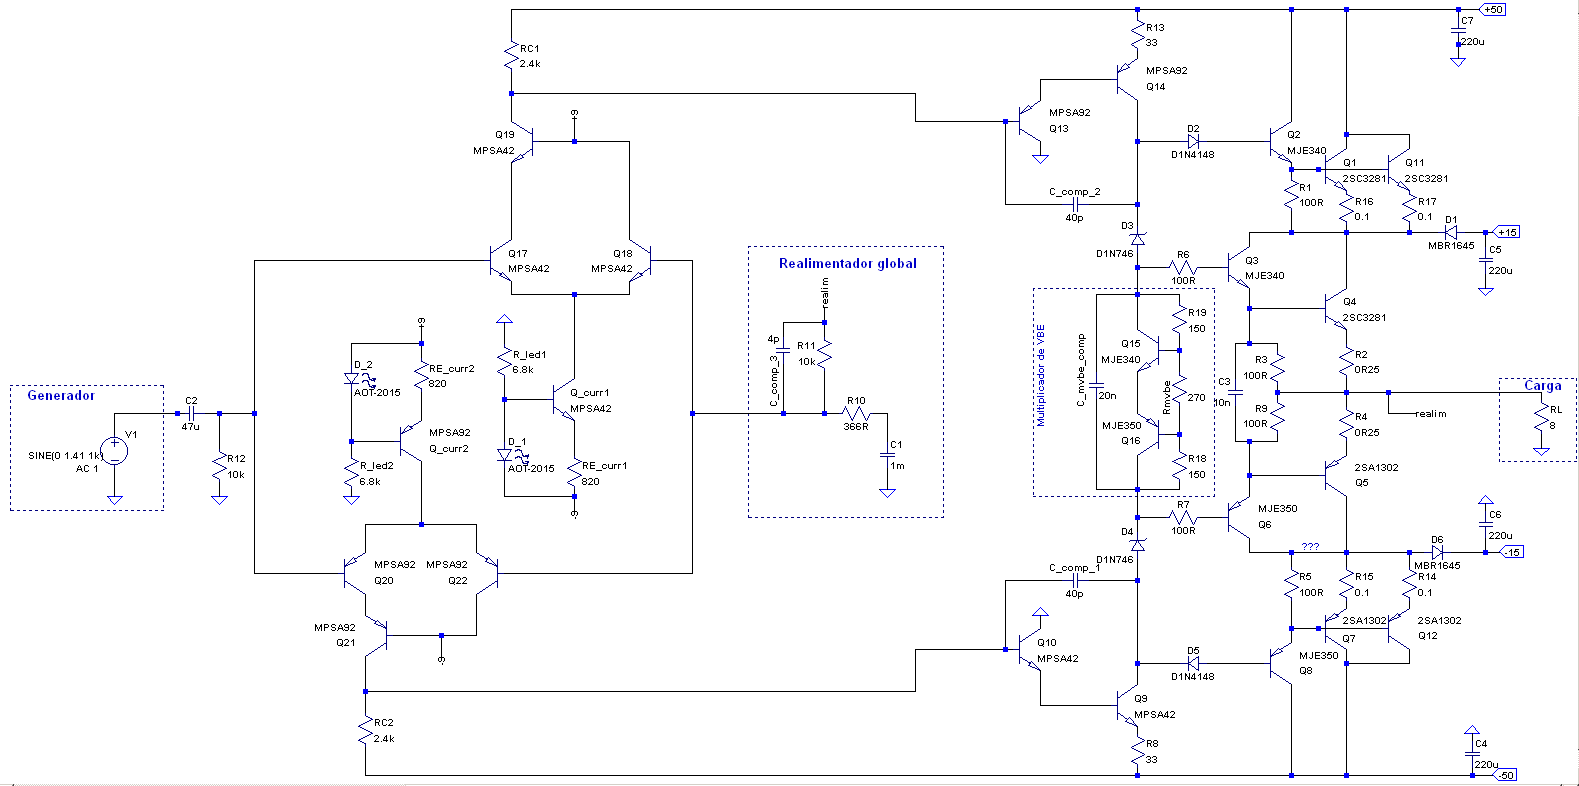
\includegraphics[width=0.75\paperheight,angle=90,origin=c]{img/circuito}
\caption{Circuito Diseñado}
\label{fig:circuito} 
\end{figure}

\subsection{Integracion}
\paragraph{Alimentación}

Se colocaron capacitores (\texttt{C4},\texttt{C5},\texttt{C6} y \texttt{C7}) en los 4 rieles de alimentación ($\pm 50V$ y $\pm 15V$) para filtrar ruidos a la entrada.

\paragraph{Etapa de entrada}

Se usó doble par diferencial para mantener la simetría total y reducir la distorsión por armónicos pares. Cada par se diseñó teniendo en cuenta que la tensión de salida de polarización debía ser estable, pues la segunda etapa no estará polarizada por una fuente de corriente. Por esto, la resistencia de carga del par diferencial (\texttt{RC1} y \texttt{RC2}) es de sólo $2.4k\Omega$, mucho menor que la resistencia dinámica de pequeña señal que le ofrece la segunda etapa ($\cong 100k\Omega$), dominando el paralelo.
Por la misma razón, se consideró de particular importancia garantizar que las corrientes de polarización por las ramas del par se independicen de posibles variaciones en la segunda etapa o del riel. Los transistores \texttt{Q19} y \texttt{Q21}, en configuración cascode con \texttt{Q17} y \texttt{Q20} cumplen justamente la función de generar esta independencia.

Se polarizó cada rama con una corriente de $\cong 1mA$. Mayor corriente no generaría una mucho mayor amplificación de la etapa, pues, para mantener una tensión de salida fija habría sido necesario reducir la resistencia de carga en igual proporción. Esta corriente se generó con una fuente hecha por un LED de $2.3V$. Este LED permitirá visualizar rápidamente posibles errores de polarización en el amplificador armado.


\paragraph{Etapa de amplificación de tensión}

Se optó por una configuración CC-EC, una para cada salida del doble par diferencial (figura~\ref{fig:vas-1}). El colector común cumple la función de ofrecer una resistencia alta a la primera etapa, independizando la polarización de los parámetros variables de los transistores de la segunda etapa. Además, aumenta la diferencia de tensión de polarización requerida entre el riel y la entrada de la etapa, lo que permite el uso de una resistencia de carga mayor en la primera etapa, mejorando su ganancia. Esta configuración, además, ofrece un alto grado de independencia de las variaciones de tensión del riel, pues todas las tensiones involucradas varían en conjunto (la única que no lo hace es masa, pero está conectada al colector de \texttt{Q13} y \texttt{Q10}, nodos de alta impedancia). 


\begin{figure}[H]
\centering
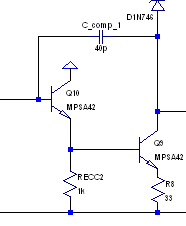
\includegraphics[width=0.3\textwidth]{img/sim/vas-1}
\caption{VAS en CC-EC del riel negativo del circuito diseñado.}
\label{fig:vas-1} 
\end{figure}

Las resistencias de emisor del EC (\texttt{R8} y \texttt{R13}) implementan realimentaciones locales que estabilizan la corriente de polarización y ganancia de la etapa. Son realimentaciones que serie-serie (muestrean corriente y suman tensión). Son de valor reducido pues al estabilizar la ganancia, la reducen. Además, la caída de tensión en estas resistencias reduce la máxima excursión de la etapa antes de que saturen los transistores. Se eligieron los valores exactos (junto con los de las cargas de la primera etapa) para que la corriente de polarización sea $\cong 25mA$.

Las resistencias \texttt{RECC2} y \texttt{RECC1} aseguran una corriente de polarización del colector común $>1.5mA$. De no existir, la polarización podría ser muy baja, y dependiente de las variabilidades del $\beta$ del transistor del EC. Esta baja corriente implicaría, además, un $r_d$ grande, y esto es indeseable: El EC es un amplificador de conductancia y, como tal, funciona mejor recibiendo una señal de entrada de baja impedancia por su base.


\paragraph{Etapa de salida}

Se usan transistores en configuración Darlington, para tener una ganancia de corriente elevada, y con transistores en paralelo en la parte de mayor potencia para repartir la corriente y disminuir la disipación en cada uno. Se colocaron las resistencias \texttt{R14}, \texttt{R15}, \texttt{R16} y \texttt{R17} de valor $0.1\Omega$ para ayudar a que se reparta de forma equilibrada la potencia entre los transistores de potencia \texttt{Q1}-\texttt{Q11} y \texttt{Q7}-\texttt{Q12}.


\paragraph{Multiplicador de $V_{be}$}


Se diseñó (figura~\ref{fig:mvbe}) con dos transistores para mantener la simetría total del circuito. La corriente de polarización de los transistores del VAS es $\cong 25mA$, y esta puede tener una excursión máxima de aproximadamente $4mA$ pico-a-pico. Es decir, el multiplicador debe lograr polarizarse con corrientes de $\cong 20mA$. Las simulaciones muestran que se logra una mayor estabilidad en la tensión si los transistores están polarizados con corrientes bajas. Por lo tanto, se eligió \texttt{Rmvbe} tal que consuma una corriente $<20mA$, pero del orden de los $mA$. Se podría haber elegido un valor más cercano a $20mA$, pero una simulación remplazando al multiplicador por un generador de tensión ideal mostró que el funcionamiento y la distorsión del circuito no se veían afectados. Por esta misma razón, no se agregaron resistencias adicionales en los colectores, que usualmente se usan para generar una caída que compense el incremento de tensión con la corriente. Puede hacerse como posible optimización.

Las resistencias \texttt{R18} y \texttt{R19} se eligieron iguales por simetría, y de valor tal que la tensión generada sea levemente superior a $2.8V$. Esto permite colocar a los transistores de salida en modo levemente A-B, reduciendo la distorsión de su etapa.


\begin{figure}[H]
\centering
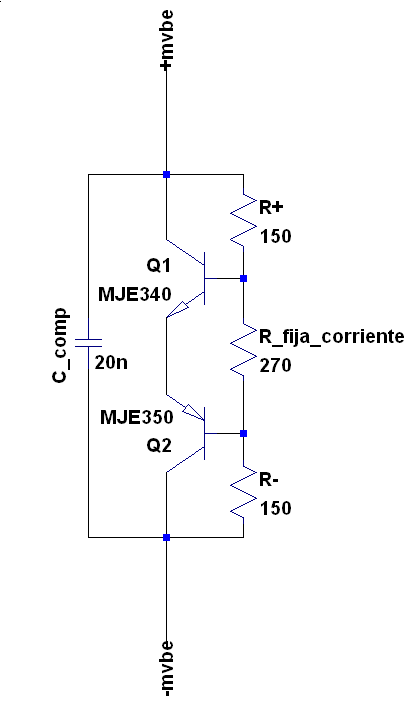
\includegraphics[height=0.3\textwidth]{img/sim/mvbe}
\caption{Multiplicador de $V_{be}$ simétrico utilizado.}
\label{fig:mvbe} 
\end{figure}

%Dice en la consigna que acá toca:
%1.Explora distintos circuitos y analiza CORRECTAMENTE su funcionamiento*
%2.Calcula CORRECTAMENTE TODOS los componentes de circuitos individuales y las
%condiciones de funcionamiento*
%3.Investiga y selecciona los componentes
%4.Valida y optimiza el diseño mediante simulaciones y mediciones, y determina todos los
%parámetros de funcionamiento de los circuitos
%5.Determina si las especificaciones del circuito son alcanzables*
%6.Realiza las simulaciones, indica y explica los circuitos simulados, los puntos de medición,
%los parámetros utilizados y los resultados obtenidos
%7.Realiza mediciones, indica y explica los circuitos implementados, las mediciones
%realizadas, los instrumentos utilizados y los resultados obtenidos*
%8.Realiza los diagramas esquemáticos con las referencias de todos sus componentes
%9.Realiza el listado de componentes indicando referencia, descripción, valor, parámetros, fabricantes y posibles proveedores para cada componente.



\subsubsection{Simulaciones}


\paragraph{THD} A continuación se muestra una tabla con los resultados del análisis de Fourier realizados con el LTSpice para entrada de $1.41V$ pico (máxima excursión, $100W RMS$) a $1kHz$. 




\begin{verbatim}
Harmonic	Frequency	 Fourier 	Normalized	 Phase  	Normalized
 Number 	  [Hz]   	Component	 Component	[degree]	Phase [deg]
    1   	1.000e+03	3.985e+01	1.000e+00	    0.00°	    0.00°
    2   	2.000e+03	3.599e-03	9.032e-05	   91.57°	   91.57°
    3   	3.000e+03	1.515e-02	3.803e-04	    1.50°	    1.50°
    4   	4.000e+03	1.144e-03	2.871e-05	   94.01°	   94.01°
    5   	5.000e+03	1.920e-03	4.817e-05	 -177.23°	 -177.23°
    6   	6.000e+03	5.374e-04	1.348e-05	  -74.65°	  -74.65°
    7   	7.000e+03	6.560e-04	1.646e-05	   14.67°	   14.67°
    8   	8.000e+03	3.168e-04	7.950e-06	  129.84°	  129.84°
    9   	9.000e+03	3.698e-04	9.279e-06	   -5.66°	   -5.66°
   10   	1.000e+04	3.239e-04	8.127e-06	   61.19°	   61.19°
...
Total Harmonic Distortion: 0.0396%


\end{verbatim}

La distorsión armónica simulada es de $0.04\%$ en la máxima excursión a $1kHz$. Una simulación similar determina que la distorsión a $10kHz$ es de $0.03\%$. A $1W$ ($4V$) de salida, y $1kHz$, la distorsión es de $0.0016\%$ y a $10kHz$, $0.002\%$. Salvo este último caso, aún no cumplen con el $0.01\%$ especificado.


En la figura~\ref{fig:distorsion-barrido} se muestra la distorsión a $1kHz$ en función de la tensión pico de salida.

\begin{figure}[H]
	\centering
	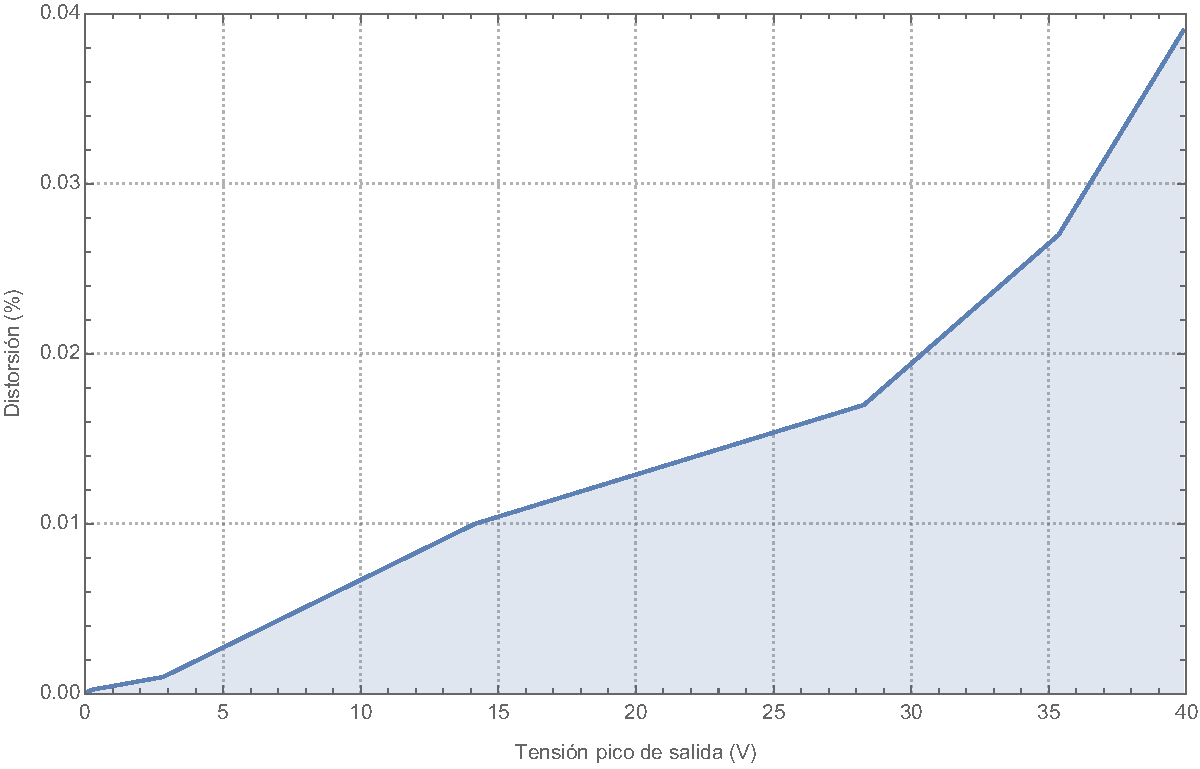
\includegraphics[width=0.6\textwidth]{img/sim/distorsion-barrido}
	\caption{Distorsión a $1kHz$ a distintos valores de tensión pico de salida.}
	\label{fig:distorsion-barrido}
\end{figure}

Los valores de distorsión bajan a potencias menors porque se reduce la distorsión por alinealidad de los transistores: mientras más chica es la excursión, más uno se encuentra en pequeña señal, y más lineal es la relación entre $v_{be}$ e $i_c$. Por otra parte, se colocó al multiplicador de $V_{be}$ de modo tal que haga funcionar a la etapa de salida en modo A-B, reduciendo la distorsión por crossover.

\paragraph{Slew Rate} Simulando una entrada escalón en el amplificador, se observa la salida de la figura~\ref{fig:slew} en la carga.

La pendiente es de $20 \frac{V}{\mu s}$. Esto es mayor a la máxima pendiende de la salida en máxima potencia a la máxima frecuencia especificada de $30kHz$, por lo que el ancho de banda de potencia cumplirá lo especificado ($15 \frac{V}{\mu s}<20 \frac{V}{\mu s}$).


\begin{figure}[H]
	\centering
	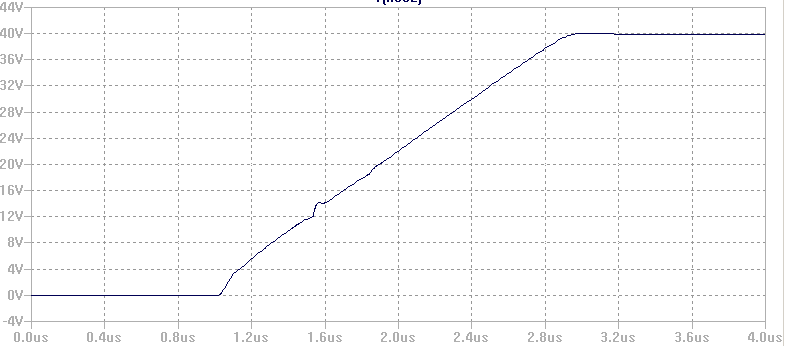
\includegraphics[width=0.6\textwidth]{img/sim/slew}
	\caption{Salida simulada frente a una entrada escalón.}
	\label{fig:slew}
\end{figure}

\paragraph{CMRR - factor de rechazo de modo común}

Un amplificador diferencial ideal debería amplificar, como dice su nombre, las diferencias entre las tensiones de entrada, e ignorar la tensión media. El parámetro CMRR mide cuan bien esto se logra, como el cociente entre la ganancia de modo común $A_c$ y la de modo diferencial $A_d$. 

\subparagraph{Modo común} Se simuló la primera etapa frente una entrada común de $100mA$ con el circuito de la figura~\ref{fig:ac} y se obtuvo la ganancia de modo común. Para cada par diferencial del doble par, cuyas salidas son \texttt{o1} y \texttt{o2} en la figura~\ref{fig:ac}, se obtuvieron $A_c^{NPN}=\frac{V_{o1}}{100mV}$ y $A_c^{PNP}=\frac{V_{o2}}{100mV}$ como la relación entre la salida (pico) correspondiente al par y la entrada común (pico). 


\begin{figure}[H]
	\centering
	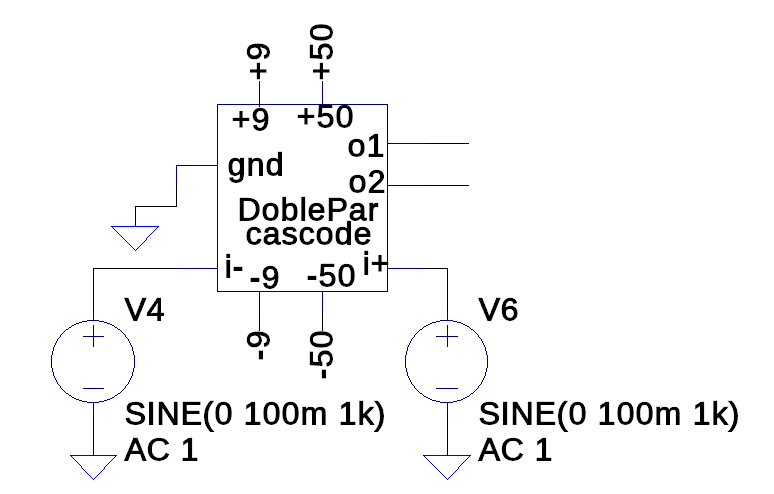
\includegraphics[height=0.2\textwidth]{img/sim/ac}
	\caption{Circuito usado para simular la amplificación de modo común.}
	\label{fig:ac}
\end{figure}

\subparagraph{Modo diferencial}

La amplificación de modo diferencial se obtuvo de forma análoga, con las fuentes de la figura~\ref{fig:ac} conectadas a contrafase. Las tensiones pico de las fuentes usadas fueron de sólo $1mV$ porque se esperaba una amplificación mucho mayor que para el caso de modo común. Es decir, $A_d^{NPN}=\frac{V_{o1}}{2mV}$, y $A_d^{PNP}=\frac{V_{o2}}{2mV}$.

\subparagraph{CMRR} El factor de rechazo es simplemente $\frac{A_d}{A_c}$, en valor absoluto.


\begin{table}[H]
\centering
\begin{tabular}{l|ll}
 & NPN & PNP \\ \hline
$A_c$ & $-56dB$ & $-59dB$  \\
$A_d$ & $31dB$ & $33dB$  \\
RRMC & $87dB$ & $92dB$  
\end{tabular}
\end{table}

\paragraph{PSRR - factor de rechazo a la fuente}

El PSRR se define como la relación entre el cambio en la tensión de alimentación y el cambio equivalente en la tensión de entrada. Idealemente este valor sería infinito.

Simulando para valores de la fuente de $+50V$ entre $40V$ y $60V$ se obtuvo:

\[ PSRR := {\Delta V_\mathrm{fuente} \over {\Delta V_\mathrm{o}}} \cdot A_d = 86dB \]



Es decir, con la ganancia de $29dB$ de este circuito, por cada $1V$ de riple en la fuente de $+50V$ se superponen aproximadamente $1.4mV$ en la salida ($86dB-29dB=57dB$ y $10^\frac{-57}{20} \cong 1.4mV $)

También, se simuló y verificó el comportamiento correcto del amplificador para una posible caída de tensión en los rieles del $10\%$: sólo se reduce la máxima excursión.

\paragraph{Resistencia de salida}  

Para la simulación de la resistencia de salida, se colocó una fuente de corriente alterna de $1A$ a la salida, con la entrada pasivada, y se capturó la tensión de salida en un barrido de frecuencias.


El circuito simulado, con una caja representando el amplificador, se observa en la figura~\ref{fig:circuito_r-out-current}.


\begin{figure}[H]
	\centering
	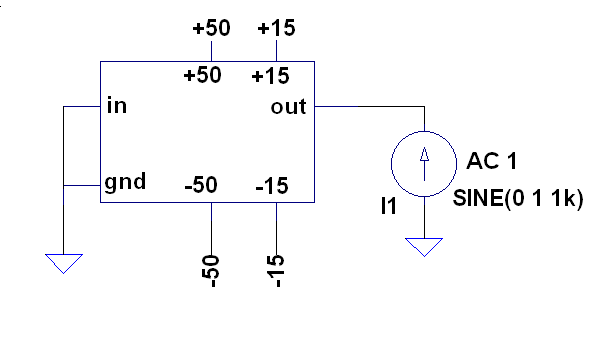
\includegraphics[width=0.6\textwidth]{img/sim/circuito-r_out-current}
	\caption{Circuito usado para simular la resistencia de salida. La caja representa al amplificador.}
	\label{fig:circuito_r-out-current}
\end{figure}

Los resultados del barrido se muestran en la figura~\ref{fig:R_out}, y un zoom en las frecuencias de trabajo especificadas en la figura~\ref{fig:R_out-zoom}.

\begin{figure}[H]
	\centering
	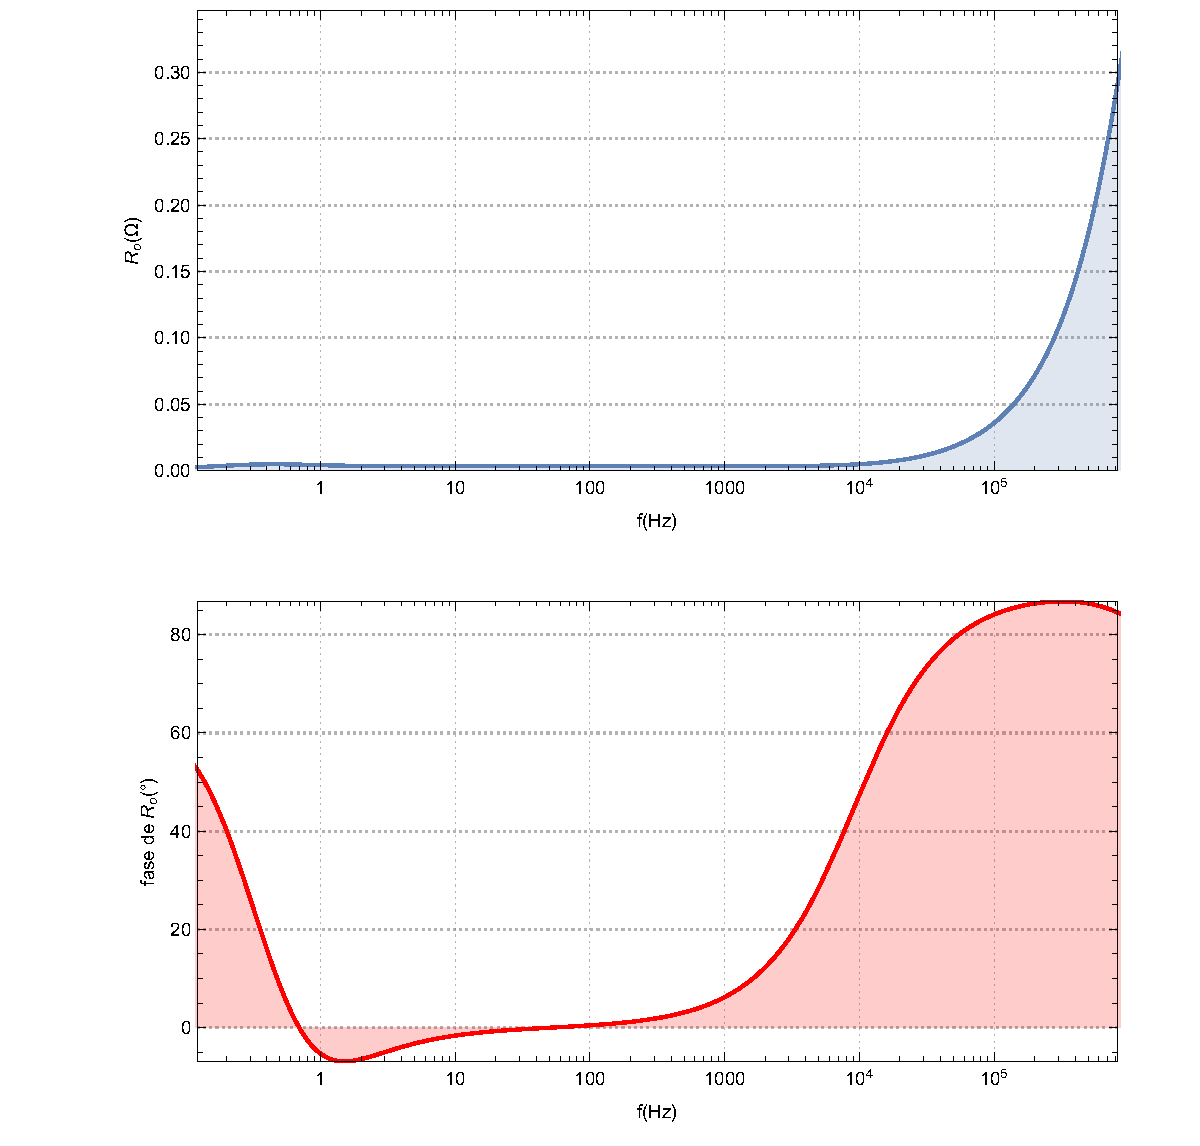
\includegraphics[width=0.6\textwidth]{img/sim/R_out}
	\caption{Barrido en frecuencias de la impedancia de salida simulada.}
	\label{fig:R_out}
\end{figure}

\begin{figure}[H]
	\centering
	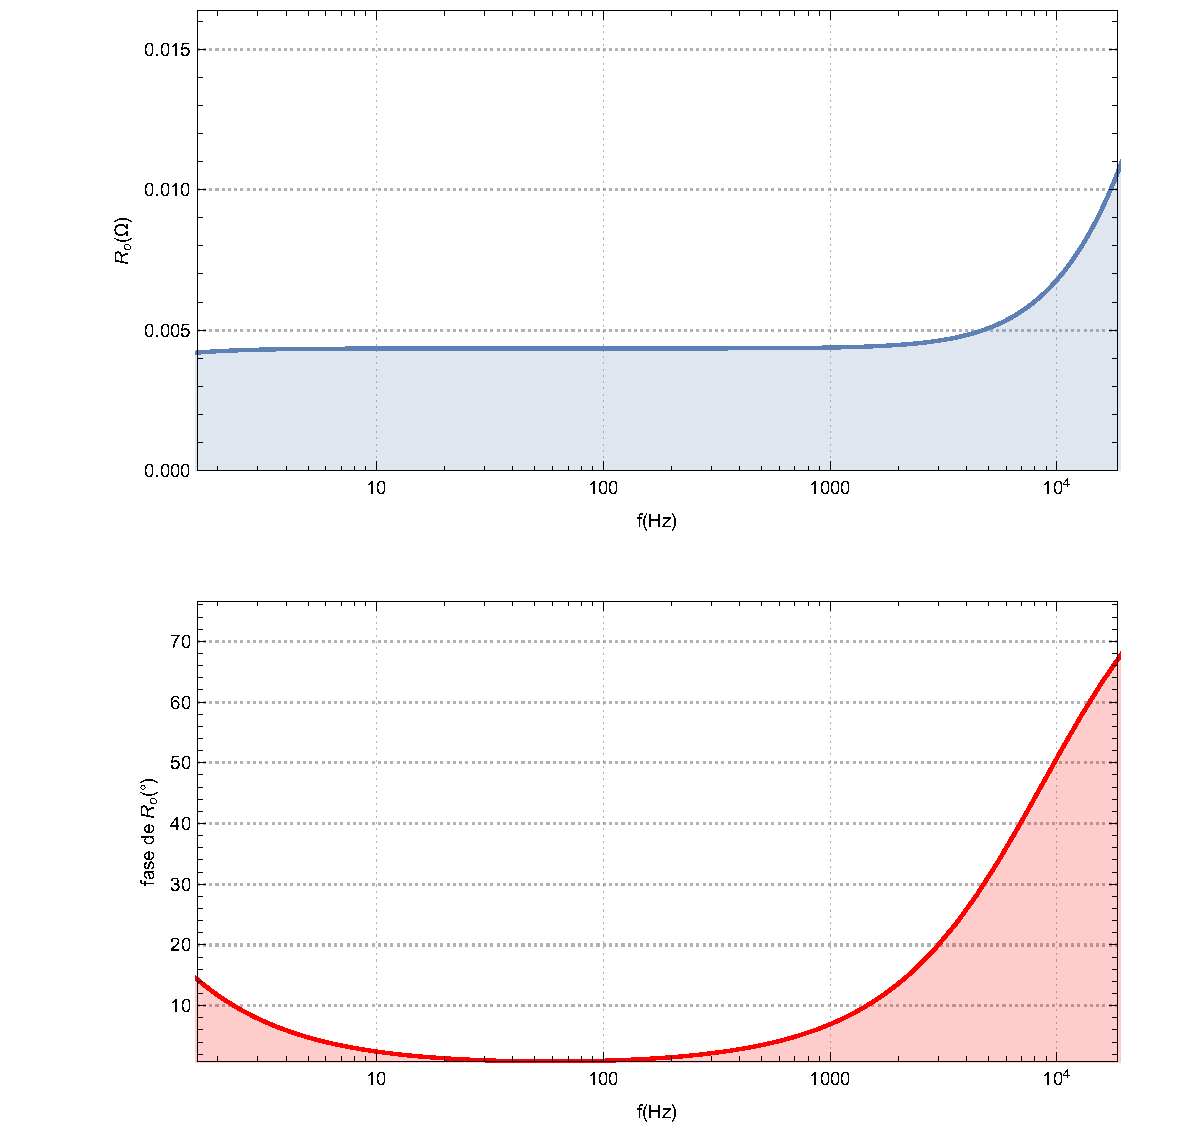
\includegraphics[width=0.6\textwidth]{img/sim/R_out-zoom}
	\caption{Barrido en frecuencias de la impedancia de salida simulada para frecuencias hasta $30kHz$.}
	\label{fig:R_out-zoom}
\end{figure}

El módulo de la media geométrica de la impedancia de salida para las frecuencias entre $1Hz-30kHz$ es $11m\Omega$.

\[R_{out}\cong 11m\Omega\]

La realimentación global serie-paralelo logra que la resistencia de salida sea muy baja, tanto que las resistencias parásitas pueden terminar siendo un factor no despreciable. Si se desprecian, el factor de amortiguamiento es de $\cong 730$, cumpliendo cómodamente con lo especificado.


\paragraph{Resistencia de entrada}

Se simuló en el cociente entre la tensión de entrada y la corriente entregadas por el generador, para un barrido de frecuencias. El módulo de la media geométrica de la impedancia para las frecuencias entre $1Hz-30kHz$ es $9.8k\Omega$.

\[R_{in}=9.8k\Omega\]

En la figura~\ref{fig:R_i} se puede ver un barrido en frecuencias de la resistencia de entrada para pequeña señal.


\begin{figure}[H]
	\centering
	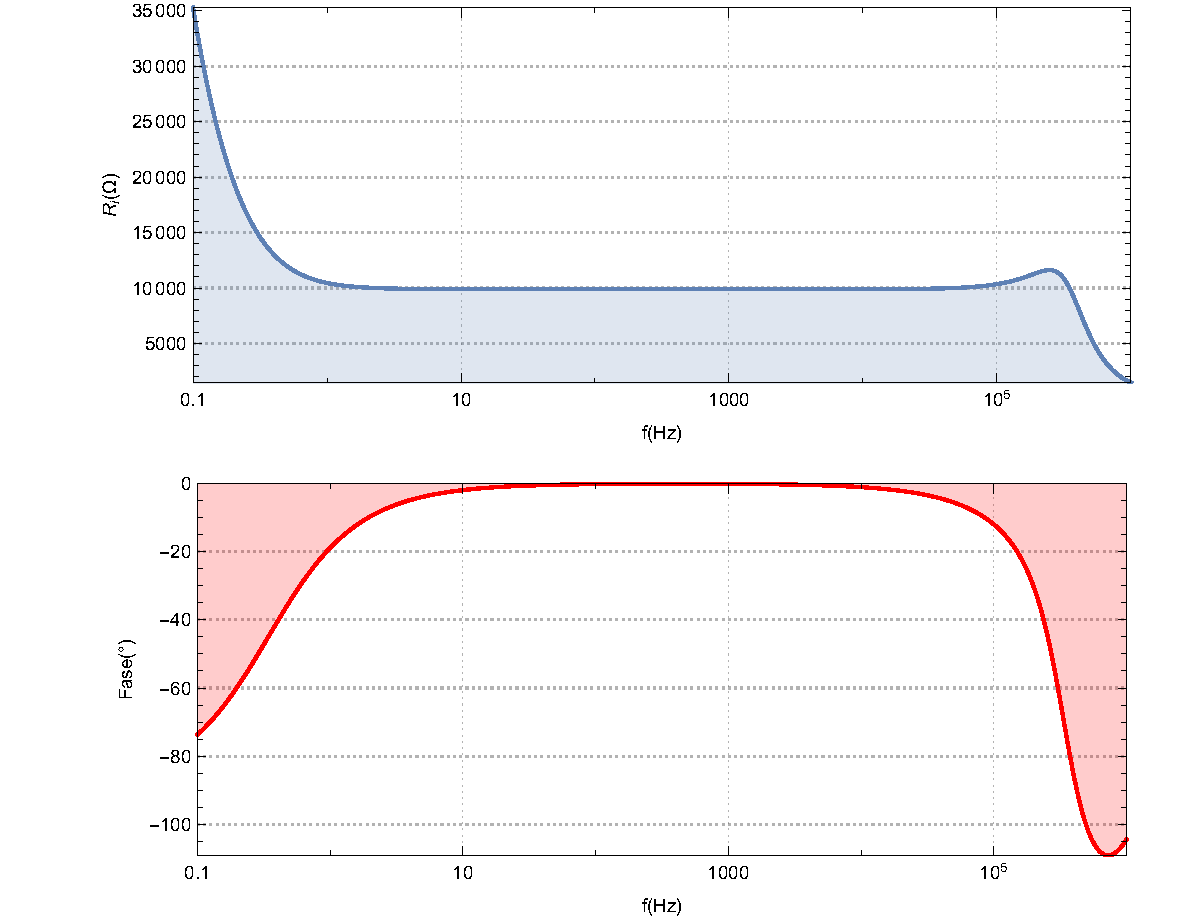
\includegraphics[width=0.6\textwidth]{img/sim/R_i}
	\caption{Resistencia de entrada. Cociente entre tensión y corriente de entrada simuladas para pequeña señal de distintas frecuencias.}
	\label{fig:R_i}
\end{figure}


% Parece baja?

\paragraph{Respuesta en frecuencia} 

Se realizó un barrido de $0.1Hz$ a $100MHz$. Se puede apreciar en la figura~\ref{fig:bode} un ancho de banda de $1.57MHz@1dB$ o $2.16MHz@3dB$.

\begin{figure}[H]
	\centering
	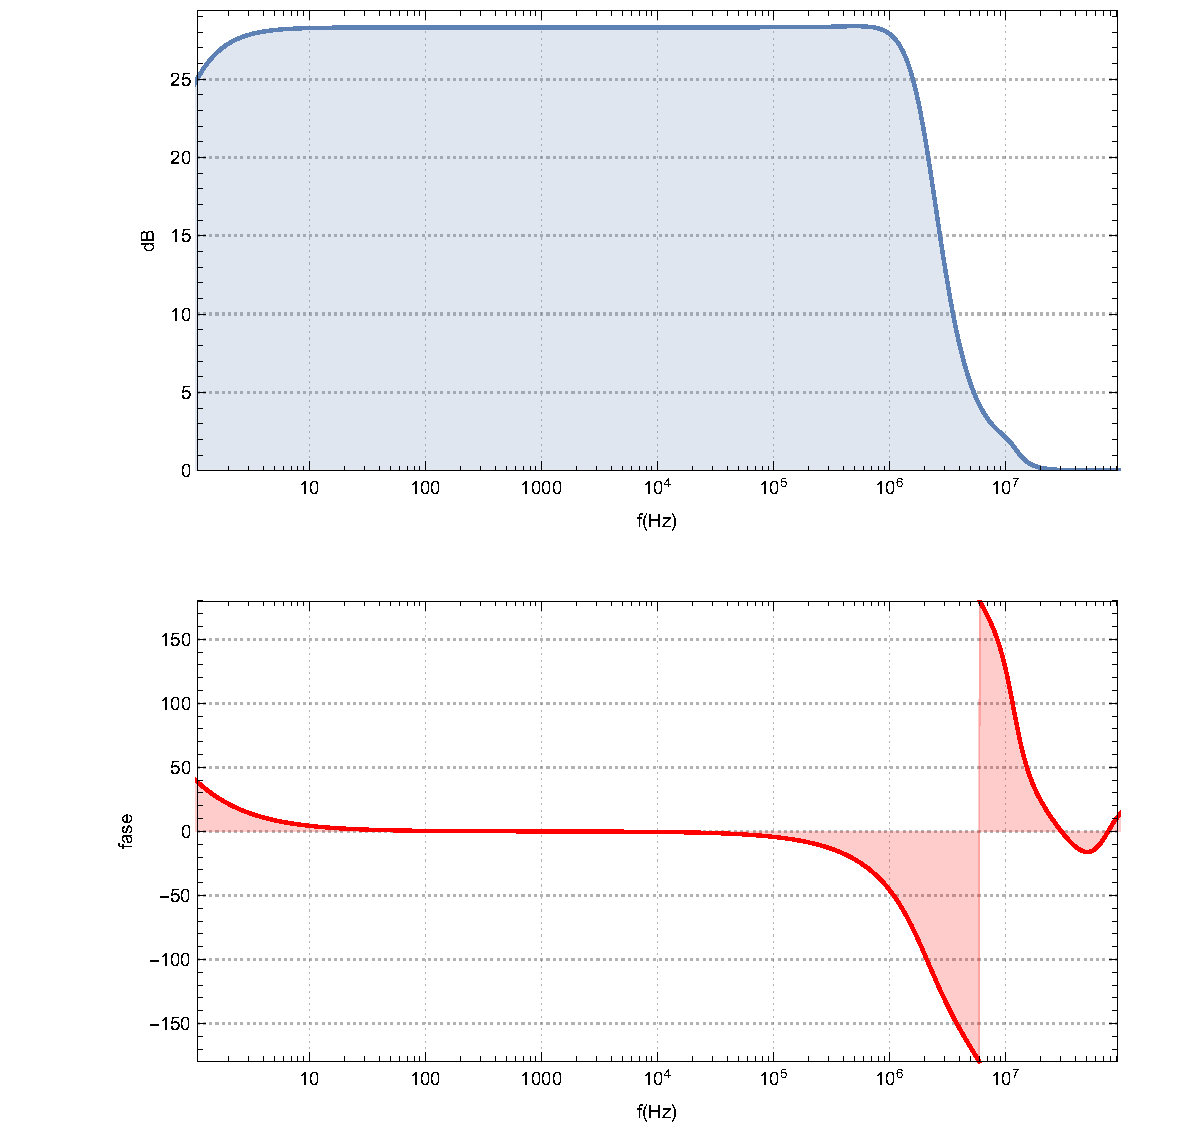
\includegraphics[width=0.6\textwidth]{img/sim/bode}
	\caption{Diagrama de Bode del amplificador a lazo cerrado simulado. El módulo, en línea llena y la fase en línea punteada.}
	\label{fig:bode}
\end{figure}



\paragraph{Ancho de banda de potencia}

Considerando el slew rate simulado de $20\frac{V}{\mu s}$, la distorsión por slew rate comenzaría a afectar a frecuencia $\frac{20\frac{V}{\mu s}}{40V \times 2\pi}\cong 80kHz$. Se puede ver en la figura~\ref{fig:distorsion-frec} cómo varía la distorsión simulada de máxima excursión con la frecuencia.


\begin{figure}[H]
	\centering
	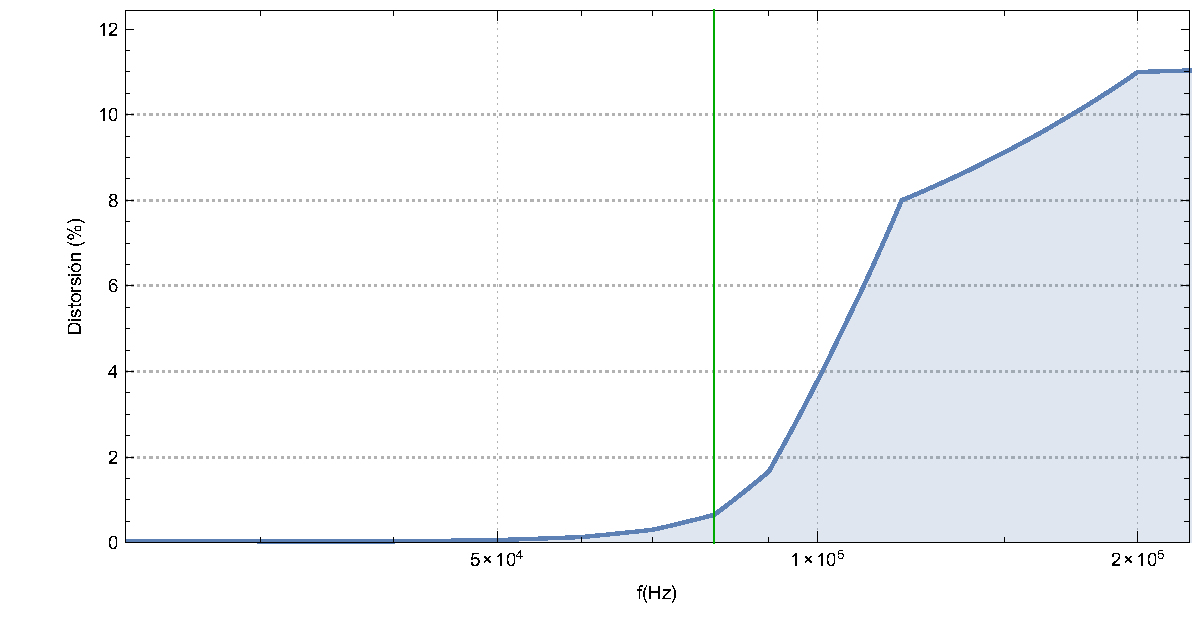
\includegraphics[width=0.6\textwidth]{img/sim/distorsion-frec}
	\caption{Distorsión a máxima excursión en función de la frecuencia. La línea verde marca la frecuencia a la cual comienza a afectar el slew rate ($80kHz$)}
	\label{fig:distorsion-frec}
\end{figure}

Tal como se preveía, en los alrededores de la frecuencia $80kHz$ la distorsión comienza a aumentar, sobrepasando valores perceptibles a simple vista mirando la forma de onda, para rápidamente estabilizarse en torno a un valor del $12\%$, que es la distorsión de una onda triangular. Esto es efecto del slew-rate.


\paragraph{Primera etapa}

En la sección de CMRR se simuló la amplificación de modo común y diferencial para la primera etapa sin carga externa. Esto es similar a la primera etapa cargada pues las resistencias de los pares diferenciales son bastante menores a las cargas que le proporciona la segunda etapa. Esto fue intencional, pues es esa resistencia la que fija la polarización de todo el circuito, y de este modo se independiza de parámetros como el $\beta$ de los transistores que puden variar con la temperatura y humedad.

Se vuelve a simular la ganancia diferencial de la primera etapa, ahora con la carga del circuito, a lazo abierto. Para esto, se coloca una capacidad de valor alto ($1F$) en la entrada realimentada del comparador (figura~\ref{fig:ala}). De este modo, no se cambiará la realimentación en polarización pero se evitará que entre señal (fijando $f_{alterna}=0$). Se obtuve una ganancia aproximada de $31dB$, como se ve en la figura~\ref{fig:1era-etapa-bode}.

\begin{figure}[H]
	\centering
	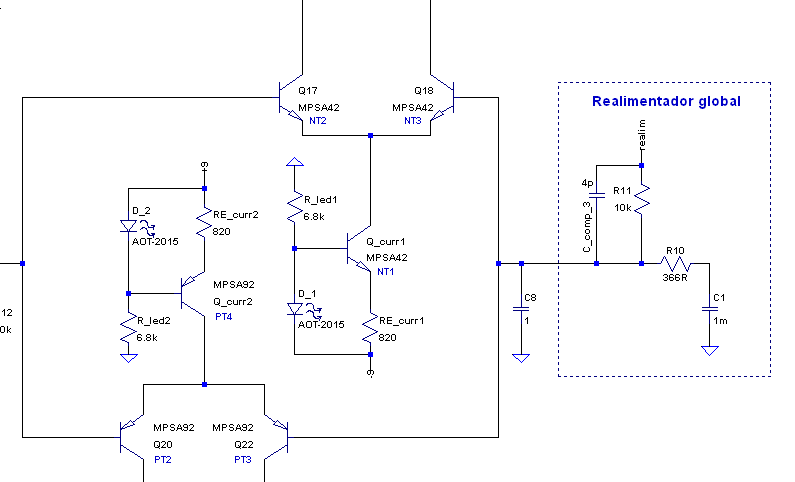
\includegraphics[height=0.4\textwidth]{img/sim/ala}
	\caption{El capacitor \texttt{C8} se agrega para anular la realimentación en señal.}
	\label{fig:ala}
\end{figure}


\begin{figure}[H]
	\centering
	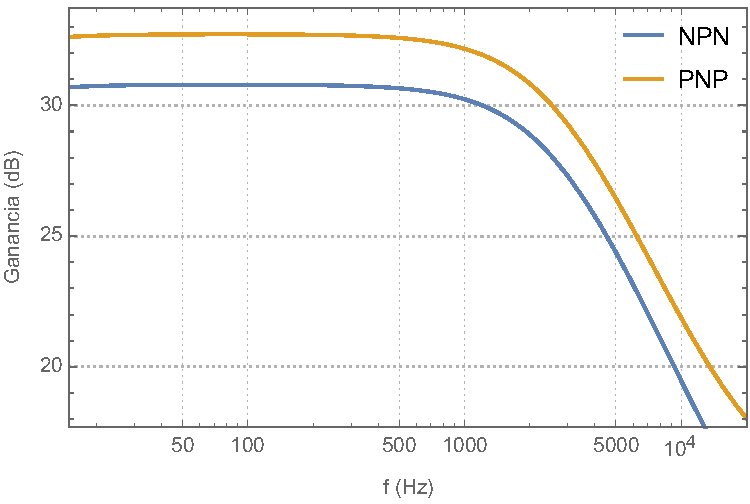
\includegraphics[height=0.4\textwidth]{img/sim/1era-etapa-bode}
	\caption{Simulación de ganancia de la primera etapa.}
	\label{fig:1era-etapa-bode}
\end{figure}

\paragraph{Segunda etapa}

El resto de la ganancia está provista por la segunda etapa, y se puede ver en la figura~\ref{fig:2da-etapa-bode}. Vale aproximadamente $55dB$.

\begin{figure}[H]
	\centering
	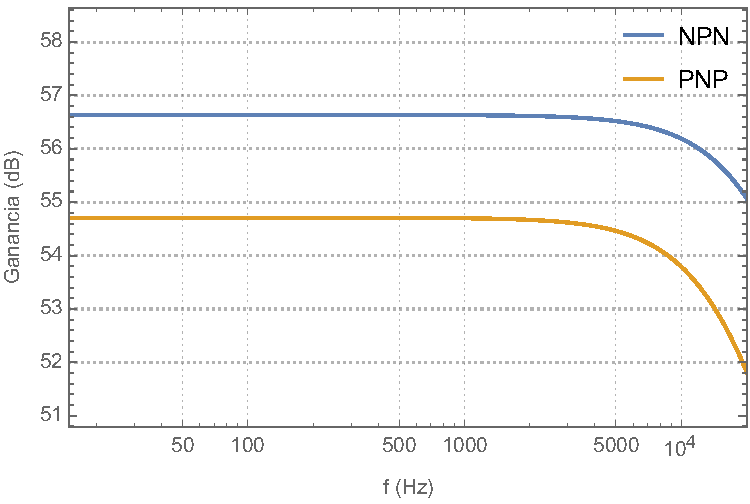
\includegraphics[height=0.4\textwidth]{img/sim/2da-etapa-bode}
	\caption{Simulación de ganancia de la segunda etapa.}
	\label{fig:2da-etapa-bode}
\end{figure}


\subsubsection{Compensación}

Un sistema realimentado puede sufrir de pérdidas de estabilidad debido al desfasaje que se produce en la señal. Si para algunas frecuencias se produce una inversión de fase y la ganancia es unitaria o mayor entonces el sistema pasa a estar realimentado positivamente para dichas frecuencias y oscila o se desestabiliza.

Para analizar la estabilidad del sistema es necesario analizar la ganancia a lazo abierto $T(j\omega)$. Un sistema adquiere la capacidad de oscilar si para una frecuencia dada $\omega_k$ se da que $T(j\omega_k)=-1$ y se vuelve inestable si $\left| T(j\omega_k) \right| > 1 \; \land \; \angle T(j\omega_k) < -180º$.

Para esta clase de análisis es útil trazar el bode de la ganancia de lazo e identificar el margen de ganancia (MG) y de fase (MF), ver figura \ref{fig:margenes}.


\begin{figure}[H]
	\centering
	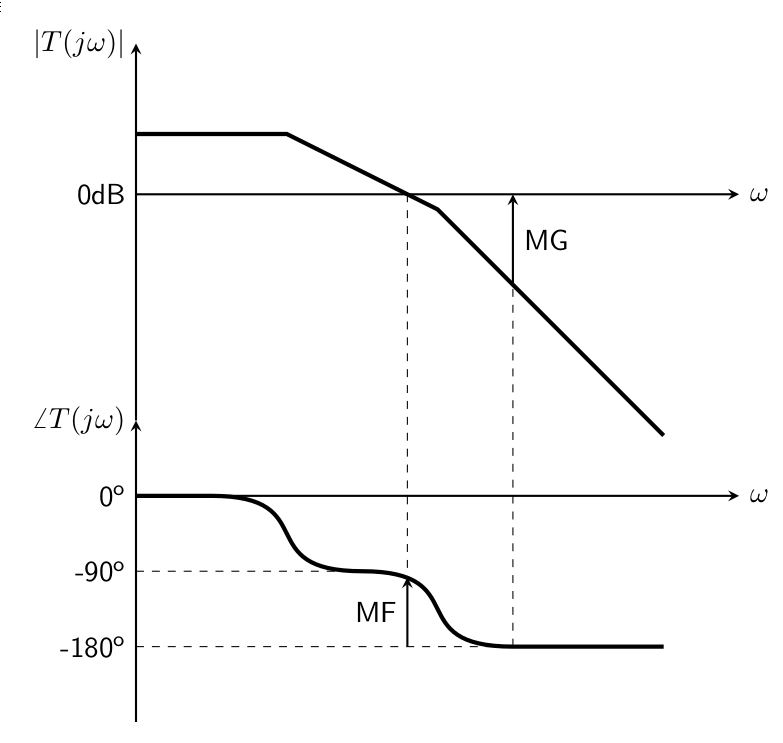
\includegraphics[height=0.4\textwidth]{img/margenes}
	\caption{Bode - margen de fase y ganancia.}
	\label{fig:margenes}
\end{figure}


Lo que representan estos margenes es lo siguiente:


\begin{description}
	\item[Margen de Ganancia] \hfill \\
		Representa la ganancia que habría que agregar (sumar en caso de dB) para volver inestable al sistema, se mide entonces la diferencia entre 0dB y la ganancia para la frecuencia en que la fase se invierte 180º. Si $\mathrm{MG} \le \mathrm{0dB}$ entonces el sistema es inestable.

	\item[Margen de Fase] \hfill \\
		Es el defasaje que habría que agregar al sistema para volverlo inestable, se mide entonces el ángulo que le resta a la fase por llegar a -180º al tener ganancia unitaria.
\end{description}

Si el margen de fase o ganancia son muy bajos o negativos, es necesario corregir, modificar el circuito para que no haya una inversión de fase en ninguna frecuencias que se amplifique en el lazo, por medio de su compensación.


Se realizó nuevamente una simulación a lazo abierto de forma análoga a la descripta en la sección anterior (figura~\ref{fig:ala}): agregando un capacitor de $1F$ en la entrada inversora del amplificador, y midiendo a la salida. Luego, a la salida se la multiplicó por $f$ para obtener una simulación de la ganancia de lazo (figura~\ref{fig:bode-la-sin-comp})

\begin{figure}[H]
	\centering
	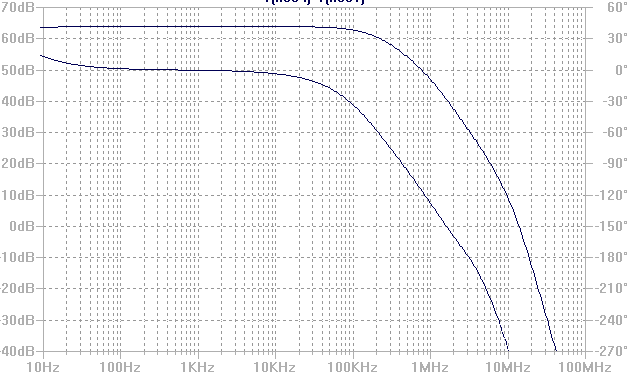
\includegraphics[height=0.4\textwidth]{img/sim/bode-la-sin-comp}
	\caption{Bode de la ganancia de lazo sin compensación. La línea inferior corresponde a la fase y la superior a la amplitud.}
	\label{fig:bode-la-sin-comp}
\end{figure}

Se puede apreciar un margen de fase negativo que es necesario compensar. El polo dominante se ubica en $180kHz$ y corresponde al nodo entre la segunda y tercera etapa: a los colectores de \texttt{Q14} y \texttt{Q9}. El margen de ganancia es de $\cong 30dB$. Desplazando al polo dominante una década y media hacia las frecuencias más bajas (hasta $5.7k\Omega$) se llega a un margen de ganancia nulo, pues un polo hace decaer la ganancia en $20dB$ por década. Sin embargo, el polo correspondiente a los nodos de entrada de la segunda etapa (bases de \texttt{Q10} y \texttt{Q13}) puede desplazarse a $5.7kHz$ con capacidades de menor valor, casi sin desplazar el polo en $180kHz$, aprovechando el efecto Miller. 
La resistencia de estos nodos está dominada por la de carga de los pares diferenciales (\texttt{RC1} y \texttt{RC2}), de valor $2.4k\Omega$. Siendo $\frac{1}{2 \pi RC}$ la frecuencia del polo, se obtiene $C\cong 11nF$. Ahora bien, si la capacidad se coloca, en vez de contra masa, contra la salida de la etapa (colectores de \texttt{Q14} y \texttt{Q9}), se puede usar una capacidad desde $20pF$, pues recordemos que la etapa tiene una amplificación de alrededor de $55dB$ o 560 veces. 

Se partió de ese valor como piso, se fue ajustando por simulación, y finalmente se colocaron capacitores (\texttt{C\_comp\_1} y \texttt{C\_comp\_2}) de $40pF$. Esto da un margen de fase de $85^{\circ}$ y un ancho de banda de $2.4MHz$. Estos capacitores limitan el slew rate, pero se observó que para valores menores a $100pF$ el slew rate se encontraba por arriba de los $7.5\frac{V}{\mu s}$ necesarios para el ancho de banda de potencia especificado, y para valores menores a $60pF$, sobre los $15V/\mu s$ especificados. Por otra parte, incrementar este capacitor reduce la ganancia de lazo en frecuencias altas y, por lo tanto, los beneficios que esto trae a la distorsión, resistencias de entrada y salida, etc. Se optó por un valor de capacidades, con margen, que podría eventualmente reducirse.

Luego, se agregó un capacitor en paralelo al realimentador (\texttt{C\_comp\_3}) para mejorar levemente estas especificaciones. Esto agrega un cero seguido de un polo. Por ejemplo, para la frecuencia del cero, la fase se incrementa en $45^{\circ}$ y la ganancia aumenta sólo en $3dB$, por lo que el ancho de banda se verá incrementado levemente y el margen de fase significativamente. Se comprobó simulando que ubicar el cero en $4MHz$ es un buen valor. Esto se obtiene con una capacidad de $4pF$ pues $\frac{1}{2 \pi 10k\Omega 4pF}\cong 4MHz$. El bode resultante de la ganancia de lazo compensado se muestra en la figura~\ref{fig:bode-la-con-comp}

\begin{figure}[H]
	\centering
	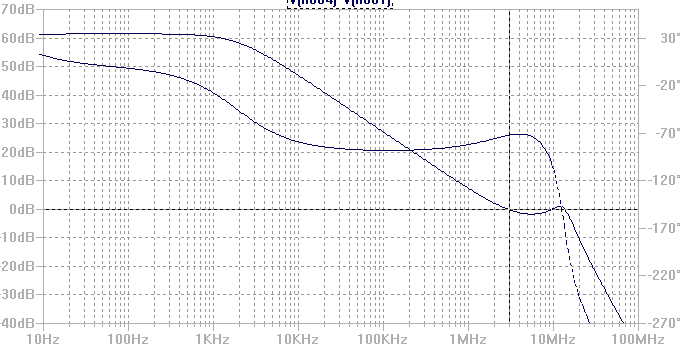
\includegraphics[height=0.4\textwidth]{img/sim/bode-la-con-comp}
	\caption{Bode de la ganancia de lazo con compensación. La línea punteada corresponde a la fase y la llena a la amplitud.}
	\label{fig:bode-la-con-comp}
\end{figure}


El margen de fase resultante ese de $105^{\circ}$ y el ancho de banda de $3MHz$, con un margen de ganancia de $3dB$. Se puede ver en la figura~\ref{fig:slew} que la respuesta al escalón no oscila.

Otra compensación se implementó para corregir el comportamiento inductivo del multiplicador de $V_{be}$ en altas frecuencias. Se compensó con el capacitor \texttt{C\_mvbe\_comp} de $20nF$.

\subsection{Redes de salida}

Usualmente, se colocan a la salida del amplificador, 2 redes, para compensar cargas inductivas o capacitivas, que pueden incluso provenir del propio cable de la salida, o del parlante. Para compensar y mantener la estabilidad en alta frecuencia frente a cargas inductivas está la red de Zobel. Para las cargas capacitivas, se usa el RL en serie.

\subsubsection{Red de Zobel}

Consiste en un RC ubicado como muestra la figura~\ref{fig:output-networks}

\begin{figure}[H]
\centering
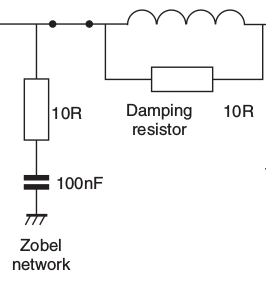
\includegraphics[width=1\textwidth]{img/output-networks}
\caption{Redes de salida típicas para compensar cargas inductivas y capacitvas.}
\label{fig:output-networks} 
\end{figure}


Otro circuito de compensación que usamos, es el denominado Red de Zobel, consiste en un circuito RC serie, colocado en paralelo a la salida, para compensar la variación de impedancia del parlante, respecto de la frecuencia. Para definir sus valores, idealmente, se debe estudiar la respuesta en frecuencia del parlante, pero, debido a que estamos armando un circuito amplificador para un parlante genérico, tomamos los valores recomendados por el libro de Douglas Self. 

\subsection{Análisis de los condicionantes de integración}

\subsubsection{Diagramas de conexionado}
El siguiente diagrama muestra como se conectaria la fuente [seccion~\ref{sec:fuente}], el amplificador y el parlante.

\begin{figure}[H]
\centering
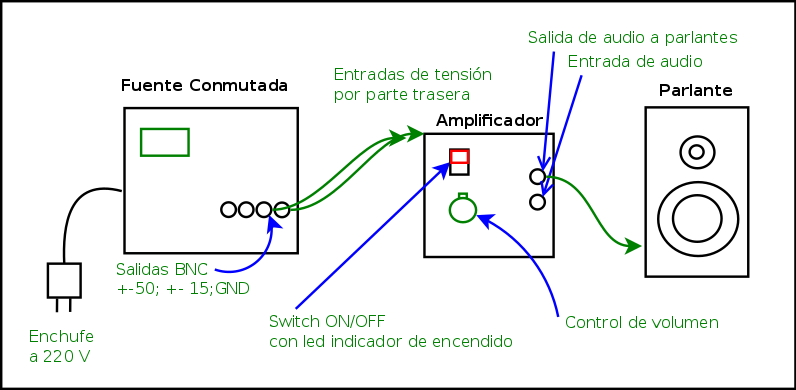
\includegraphics[width=1\textwidth]{img/integracion/diagrama_completo}
\caption{Diagrama completo}
\label{fig:diag_completo} 
\end{figure}

El la siguiente imagen se muestra el coneccionado interno del amplificador en si con los disipadores calculados [seccion~\ref{sec:disipadores}].

\begin{figure}[H]
\centering
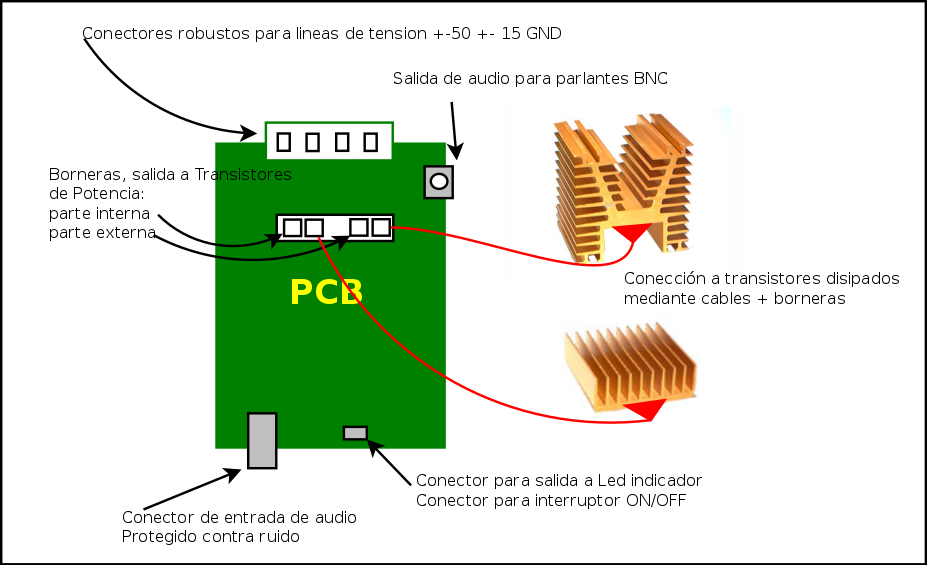
\includegraphics[width=1\textwidth]{img/integracion/diagrama_interno}
\caption{Diagrama interno}
\label{fig:circuito} 
\end{figure}




\subsubsection{Disipación de Calor}
\label{sec:disipadores}
\begin{figure}[H]
    \centering
    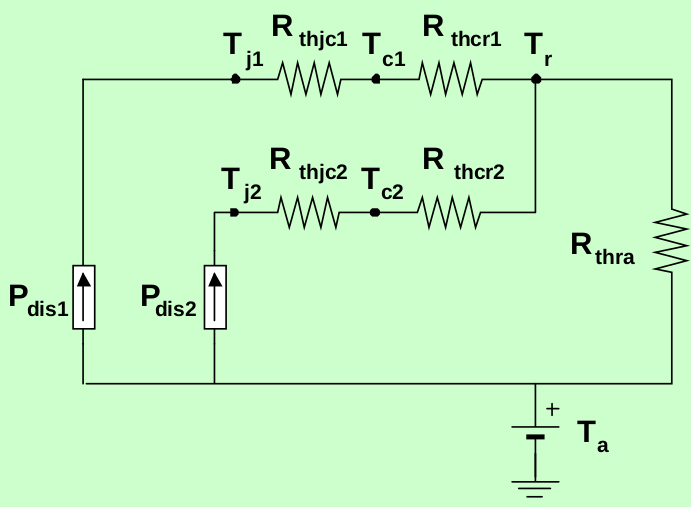
\includegraphics[height=0.4\textwidth]{img/calculo_disipador}
    \caption{Modelo termico estacionario.}
    \label{fig:disipadores}
\end{figure}

En el peor caso, los transistores de potencia 2SC3281 de la etapa de salida y su par complementario 2SA1302
disipan cada uno 18 W, ya que los mismos se utilizan en paralelo.

\begin{equation*}
T_r = R_{thra} * (P_{dis1}+P_{dis2}) + T_a
\end{equation*}

\begin{equation*}
T_r = T_{juntura_{N}} - (R_{t_{j-case}}+R_{t_{c-heat}})*P_{disN}
\end{equation*}

\begin{equation*}
T_r = 130°C - (0.85 °C/W + 0.1 °C/W)*(18*2 W) = 95.8 °C
\end{equation*}

\begin{equation*}
95.8°C = R_{thra}*(18*2*2 W) + 40°C
\end{equation*}

\begin{equation*}
R_{tha} = 0.77 °C/W
\end{equation*}

En la  parte interna de la etapa de salida, tenemos que en el peor caso se disipan 3.25  W por cada transistor.
Haciendo las mismas cuentas con otros valores.


\begin{equation*}
T_r = 120°C - (6.25°C/W + 0.1°C/W)*(3.25W) = 99.36 °C
\end{equation*}

\begin{equation*}
R_{tha} = 9.13 °C/W
\end{equation*}

\paragraph{Disipadores elegidos:}

Para la parte externa de la salida ZD-23 0.65°C/W , elegimos este modelo porque nos da un poco de margen.

\begin{figure}[H]
    \centering
    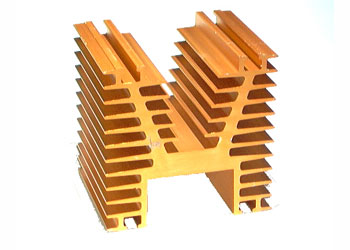
\includegraphics[height=0.4\textwidth]{img/zd23.jpg}
    \caption{Disipador ZD-23}
    \label{fig:diszd23}
\end{figure}


Para parte interna ZD-14 2°C/W, si bien solo necesitamos 9°C/W , elegimos este modelo porque nos da mas margen:

\begin{figure}[H]
    \centering
    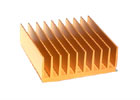
\includegraphics[height=0.4\textwidth]{img/zd14.jpg}
    \caption{Disipador ZD-14}
    \label{fig:diszd14}
\end{figure}

\subsubsection{Fuentes Conmutadas}
\label{sec:fuente}

En nuestro proyecto como ya acordamos vamos a utilizar la fuente conmutada realizada por el grupo Arias-Caracciolo-Luna.
A continuación se detallan las especificaciones basicas de la misma:

\begin{itemize}
\item{Tensión nominal de entrada: 220 V AC rms}
\item{Rango de tension de entrada: 176 V AC rms − 242 V AC rms}
\item{Rango de frecuencia de entrada: 45 Hz − 60 Hz}
\item{Tension nominal de salida:$ V_{OUT} = ± 15 V$ , $V_{OUT} = ± 50 V$}
\item{Rango de corriente de carga: Para ± 50 V : 2,5 A , Para ± 15 V : 0,7 A , Minima corriente de carga: 0 A}
\item{Potencia de entrada sin carga: Menor a 5 W para todo el rango de tensión de entrada.}
\item{Potencia de salida: Para el limite superior de la corriente de carga es 125 W}
\item{Rendimiento: Mayor a $70\%$}
\item{Protecciones de sobretensión a ± 60 V (para las salidas de ± 50 V ) y a ± 20 V (paralas salidas de ± 15 V )}
\item{Protección de cortocircuito: Clamp.}
\item{Factor de rizado (ripple): Para todas las salidas es menor a 300 mV p−p}
\item{Estabilidad a largo plazo: Tensión de ruido a la salida: Menor al $5\%$}
\item{Tipo/s de conector/es de salida: Banana hembra de 4 mm  (tipo RC170). Fijados al chasis de montaje}
\end{itemize}


%     Requerimientos Eléctricos ( Seguridad eléctrica y 
%Compatibilidad electromagnética), 
%Mecánicos (Vibraciones y Rigidez) y Térmicos (Disip
%ación de los componentes) 

 %    Definición de módulos 

%     Diseño de los Circuitos impresos 

%    Guía de localización de los componentes 

%     Diagrama de conexionado 

%     Dimensionamiento del conexionado 

%     Dimensionamiento y forma de la estructura o gabinete 

%     Dimensionamiento y posición de los puntos de fijación 

%    Diseño de los mecanismos de disipación 

%     Detalles de ensamblado y montaje 

%     Diagramas esquemáticos 

%     Listado de partes  

%     Listado de proveedores 

%     Pruebas funcionales y ambientales 

%     Análisis de modo y efecto de falla de los componentes 

%     Análisis de confiabilidad de los componentes 

%     Optimización 
\subsubsection{Capacitancias parasitas}

Debida al uso de cables:
\newline
\newline
Como se vio en el diagrama del conexionado, se van a utilizar cables para conectar el PCB con los transistores disipados, esto no es lo mejor, ya que introduce capacitancias parasitas. Segun el paper de Harry E. Green \footnote{Harry E. Green, A Simplified Derivation of the Capacitance of a Two-Wire Transmission Line, IEEE Transactions on Microwave Theory and Techniques, Vol. 47, No. 3, March 1999, p. 365-366.} la capacitancia introducida por 10 cm de cable aproximadamente a 1cm de separacion es de 1pF.

Para eliminar esta capacitancia y eliminar ruido ambiente tenemos pensado usar cable trenzado, forrado en malla metalica.

Como el de la siguiente imágen:

\begin{figure}[H]
    \centering
    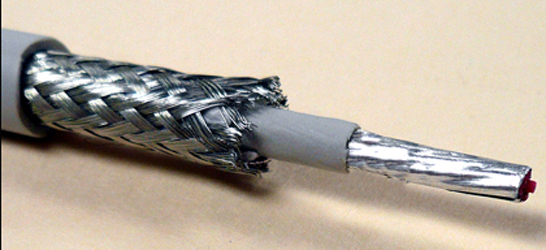
\includegraphics[height=0.31415\textwidth]{img/cable_malla_trenzada.jpg}
    \caption{Cable trenzado con malla metalica.}
    \label{fig:cable_malla}
\end{figure}



Por pistas y planos en PCB:
\newline
\newline
A la hora de diseñar el PCB se tuvieron en cuenta muchas de las tecnicas para reducir estos efectos. Sin embargo estos efectos no se pueden evitar al 100\%. Esos efectos deberian ser minimos; los mismos van a ser medidos y compensados en el momento de tener el PCB fabricado.

\newpage

\subsubsection{Lista de materiales}

\begin{table}[h!]
\centering
\caption{Lista de materiales}
\label{label}
\begin{tabular}{@{}lllllll@{}}
\toprule
Referencia            & Cantidad & Potencia  & Tensión   &  Material  & Valor    & Tolerancia \\ \midrule
RC2;RC1               & 2        &  0.25W    &           &  metal film& 2.4k     & 1\% \\
R10                   & 1        &  0.25W    &           &  metal film& 366R     & 1\% \\
C1                    & 1        &           & 65V       &  poliester & 1m       & 5\% \\
R13;R8                & 2        &  0.25W    &           &  metal film& 33R      & 1\% \\
Q14;Q13               & 2        &           &           &            & MPSA92   &     \\
Q10;Q9                & 2        &           &           &            & MPSA42   &     \\
Rmvbe1                & 1        &  0.25W    &           &  metal film& 270R     & 1\% \\
RV2                   & 1        &  0.25W    &           &  metal film& POT      &     \\
JP2;JP4;JP5;JP1;JP3   & 5        &           &           &            & JUMPER   &     \\
D3;D4                 & 2        &           &           &            & D1N746   &     \\
Q3;Q15;Q2             & 3        &           &           &            & MJE340   &     \\
R6;R7;R3;R9;R1;R5     & 6        &  0.25W    &           &  metal film& 100R     & 1\% \\
Q16;Q6;Q8             & 3        &           &           &            & MJE350   &     \\
R19;R18               & 2        &  0.25W    &           &  metal film& 150R     & 1\% \\
C3                    & 1        &           &           &  ceramico  & 10n      & 2\% \\
D2;D5                 & 2        &           &           &            & D1N4148  &     \\
Q1;Q4;Q11             & 3        &           &           &            & 2SC3281  &     \\
Q7;Q20;Q12            & 3        &           &           &            & 2SA1302  &     \\
R4;R2                 & 2        &  2W       &           &  porcelana & 0R25     & 1\% \\
D13                   & 1        &           &           &            & D        &     \\
D1                    & 1        &           &           &            & MBR1645  &     \\
R11;R12               & 2        &  0.25W    &           &  metal film& 10k      & 1\% \\
C4;C7                 & 2        &           & 65V       &  ceramico  & 220u     & 2\% \\
C5;C6                 & 2        &           & 25V       &  ceramico  & 220u     & 2\% \\
C\_mvbe\_comp1        & 1        &           &           &  ceramico  & 20n      & 2\% \\
C\_comp\_1;C\_comp\_2 & 2        &           &           &  ceramico  & 40p      & 2\% \\
T3;T4;T7;T6;T8;T5     & 6        &           &           &            & TORNILLO &     \\
R15;R14;R17;R16       & 4        &  2W       &           &  porcelana & 0R1      & 1\% \\
C\_comp\_3            & 1        &           &           &  ceramico  & 4p       & 2\% \\
U1                    & 1        &           &           &            & MMPQ2222A (SMD)& \\
R\_led1;R\_led2       & 2        &  0.25W    &           &  metal film& 6.8k     & 1\% \\
D\_1;D\_2             & 2        &           &           &            & LED      &     \\
R\_curr1;R\_curr2     & 2        &  0.25W    &           &  metal film& 820R     & 1\% \\
U2                    & 1        &           &           &            & MMPQ2907A (SMD) & \\
C2                    & 1        &           &           &  ceramico  & 47u      & 2\% \\
U4                    & 1        &           &           &            & LM7909CT &     \\
U3                    & 1        &           &           &            & LM7809CT &     \\
Rzobel1               & 1        &  0.25W    &           &  metal film& 10R      & 1\% \\
Czobel1               & 1        &           &           &  poliester & 100n     & 5\% \\ 
Disipador ZD23        & 1        &           &           &  aluminio  & 0.65°C/W &     \\  
Disipador ZD14        & 1        &           &           &  aluminio  & 2°C/W    &     \\ \bottomrule
\end{tabular}

\end{table}



\newpage
\subsubsection{Diseño PCB}

\begin{figure}[H]
    \centering
    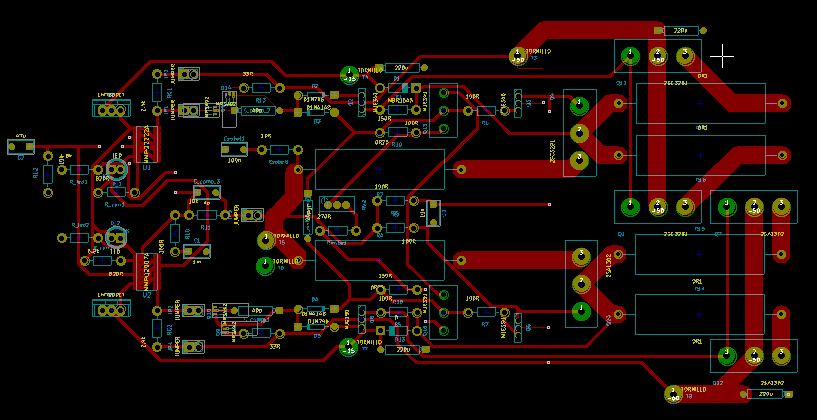
\includegraphics[height=0.4\textwidth]{img/PCB/PCB_kicad}
    \caption{Diseñando en programa Kicad}
    \label{fig:pcb1}
\end{figure}

\begin{figure}[H]
    \centering
    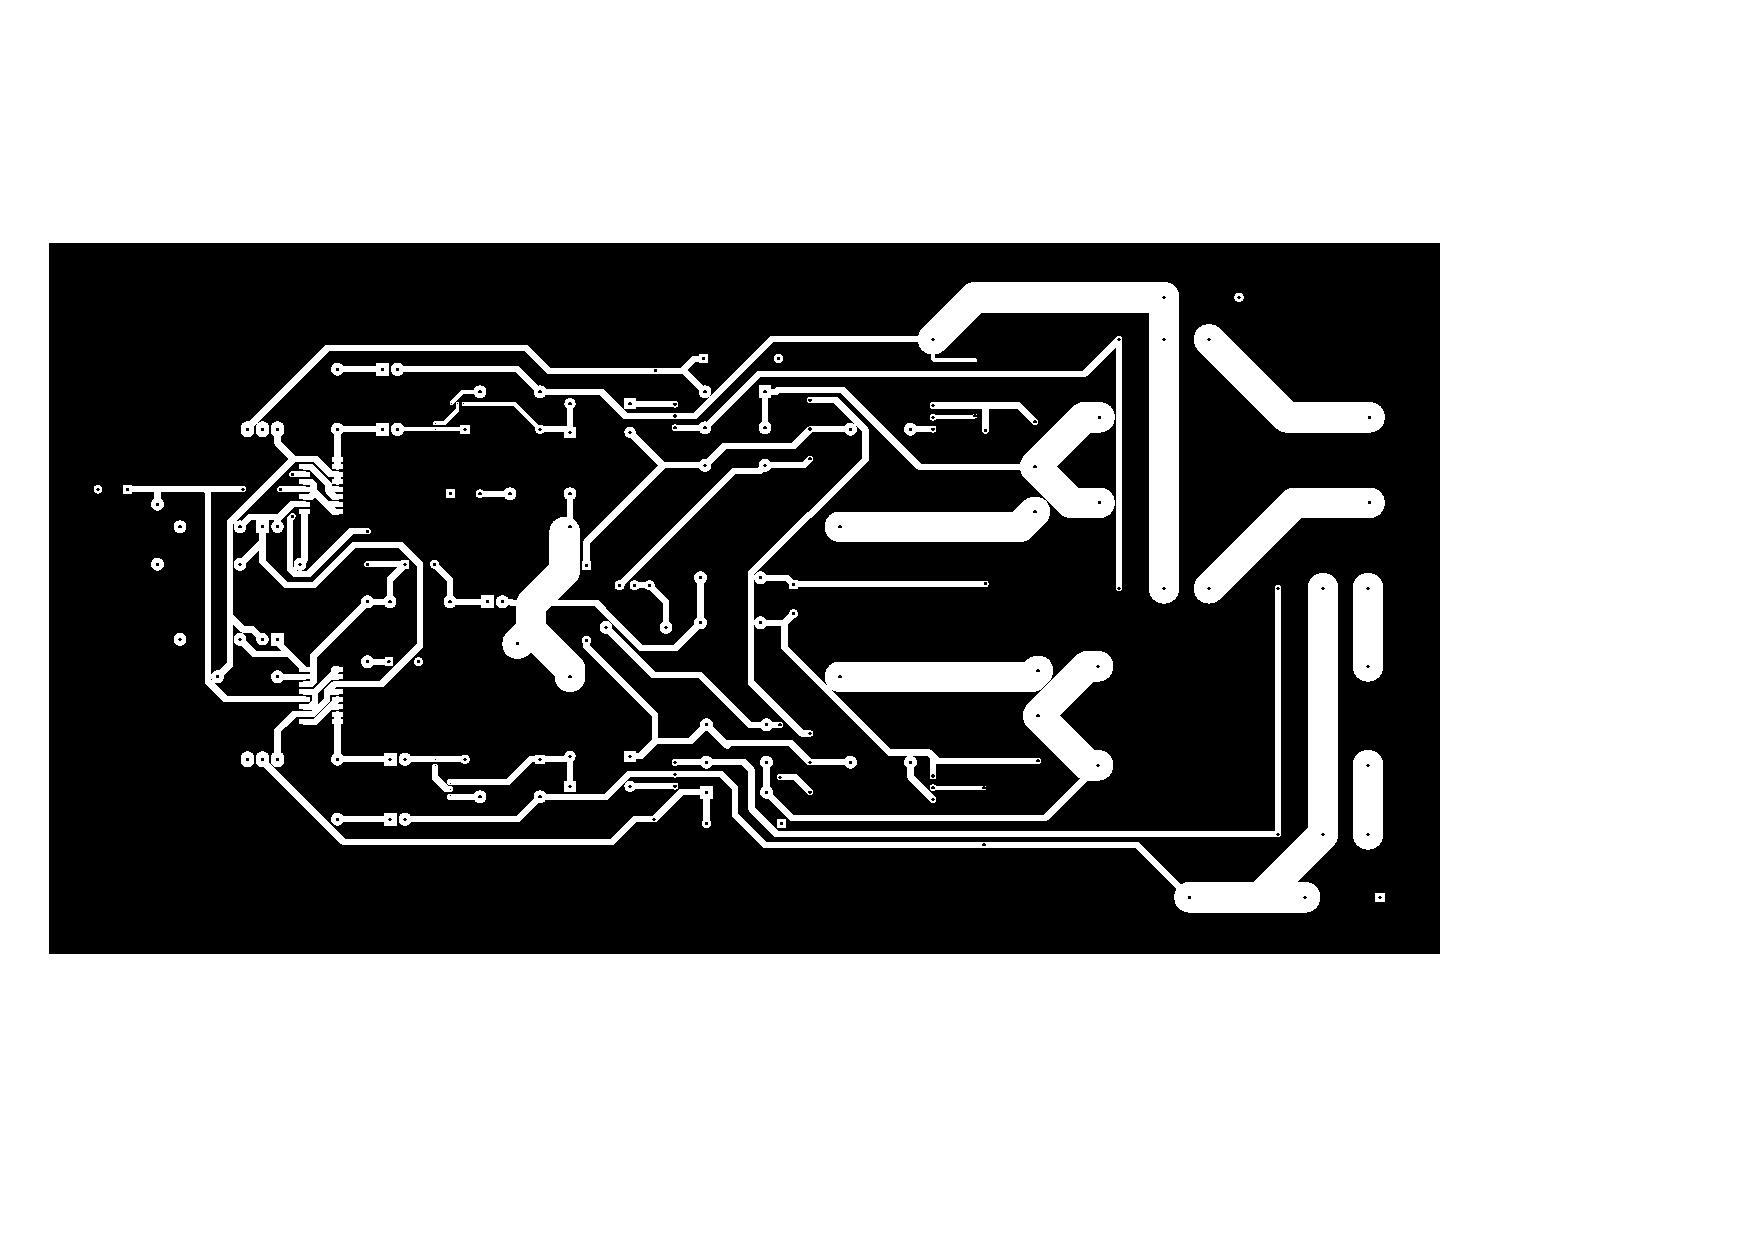
\includegraphics[height=0.7\textwidth]{img/PCB/amplificador-F.pdf}
    \caption{PCB, front}
    \label{fig:pcb2}
\end{figure}

\begin{figure}[H]
    \centering
    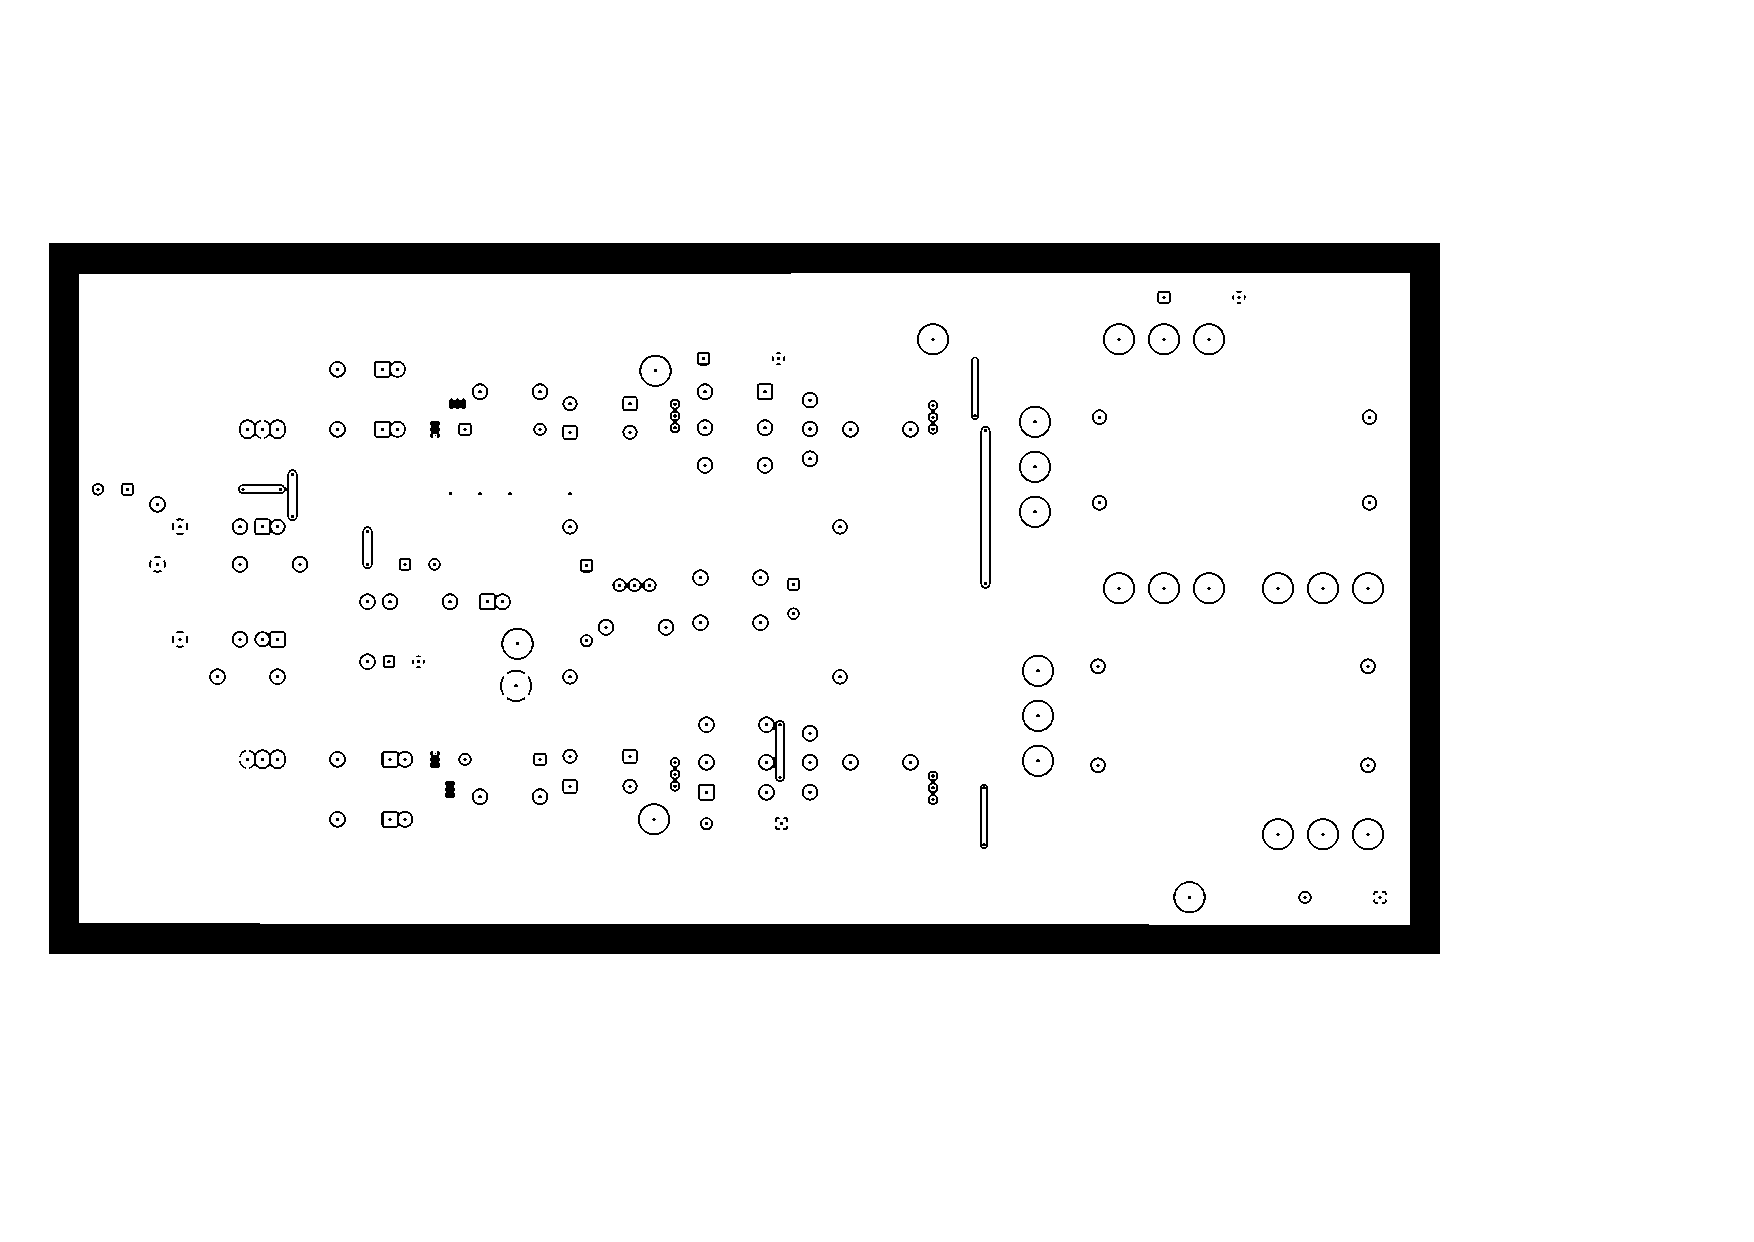
\includegraphics[height=0.7\textwidth]{img/PCB/amplificador-B.pdf}
    \caption{PCB, back}
    \label{fig:pcb3}
\end{figure}

\section{Grado de avance}

Hasta el momento, hemos elegido las configuraciones de las distintas etapas, realizamos los cálculos para hallar los valores de realimentación, resistencias para el embalamiento térmico y los disipadores para los transistores; realizamos simulaciones del circuito.

\section{Dificultades encontradas}


Para el desarrollo del proyecto, nos encontramos con varios obstáculos. En el primer diseño que realizamos, nos encontramos con una disparidad en las corrientes del par diferencial, que resolvimos comprando transistores de más, midiendo sus parámetros $\beta$, y agrupándolos para poder trabajar con valores apareados. Otra solución que encontramos, y que aplicaremos en esta versión del circuito, es utilizar transistores integrados, que asegura que todos los transistores tengan las mismas propiedades, y estén apareados. Esto también equilibraría más las amplificaciones en modo diferencial de los comparadores NPN y PNP.

La simulación de distorsión se hacía con pocos períodos en el LTSpice y, por cuestiones numéricas, eso parece resultar en valores de distorsión mucho menores a los que devuelve simulando con más períodos. Por otra parte, para valores de distorsión pequeños, se requiere un parámetro de paso máximo bastante reducido o el LTSpice sobreestima la distorsión. Se pasó mucho tiempo creyendo que el diseño resultaba en valores satisfactorios o insatisfactorios de distorsión hasta que se descubrió esto.

En un principio, la primera etapa estaba diseñada con cargas activas. Esto simulaba a veces correctamente, pero la polarización de todo el circuito resultaba poco estable e implicó el rediseño de la etapa con resistores.


\section{Resumen de actividades a desarrollar}

Habiendo establecido todo lo anterior, queda ver cómo mejorar el circuito para lograr mejores valores de distorsión. Luego procederemos con el armado del circuito, verificando el correcto funcionamiento de las etapas, durante el armado de la placa, y luego tendremos que revisar que esté andando correctamente, y que cumpla con las parámetros que propusimos. Finalizado esto, procederemos a realizar las mediciones pertinentes.

Una vez hechas las mediciones tenemos pensado agregarle a nuestro amplificador las siguientes mejoras:
\begin{itemize}
\item{Proteccion contra cortocircuito y cargas menores}
\item{Control de volumen}
\item{Carcaza protectora}
\item{Integracion compatible con fuente conmutada de grupo Arias-Caracciolo-Luna}
\item{Plug de entrada para audio con carcaza metalica contra ruidos}
\end{itemize}
\end{document}
